\documentclass[french]{scrartcl}
\usepackage[T1]{fontenc}
% $Id: vi-ref.tex,v 1.9 2004/09/28 18:19:11 dbindner Exp $
% Copyright 2002-2005 Donald Bindner
% This program is free software; you can redistribute it and/or
% modify it under the terms of the GNU General Public License
% as published by the Free Software Foundation; either version 2
% of the License, or (at your option) any later version.
% 
% This program is distributed in the hope that it will be useful,
% but WITHOUT ANY WARRANTY; without even the implied warranty of
% MERCHANTABILITY or FITNESS FOR A PARTICULAR PURPOSE.  See the
% GNU General Public License for more details.
% 
% You should have received a copy of the GNU General Public License
% along with this program; if not, write to the Free Software
% Foundation, Inc., 59 Temple Place - Suite 330, Boston, MA  02111-1307, USA.
\usepackage{babel}
\addto\extrasfrench{\providecommand{\og}{\leavevmode\flqq~}\providecommand{\fg}{\ifdim\lastskip>\z@\unskip\fi~\frqq}}
\usepackage{multicol}
\usepackage[utf8x]{inputenc}
\usepackage{array}
\usepackage{tabularx}
\usepackage{booktabs}
\usepackage{amsthm}
\usepackage{amsmath}
\usepackage{amssymb}
\usepackage[dvipsnames]{xcolor}
\usepackage{enumitem}
\usepackage{listings}
\usepackage{tabularx}
\usepackage{verbatim}
\usepackage{moreverb}
\usepackage{fancyvrb}
\usepackage{graphicx}
\usepackage{subfig}

\lstset{language=C,
	 	basicstyle=\ttfamily,
		keywordstyle=\ttfamily\textcolor{RubineRed},
		identifierstyle=,columns=fullflexible,
		commentstyle=\textcolor{OliveGreen},
		showstringspaces=false, breaklines=true,tabsize=4}

\setlength{\textheight}{7.8 in}
\setlength{\textwidth}{10 in}
\setlength{\hoffset}{-2 in}
\setlength{\voffset}{-1 in}
\setlength{\footskip}{4 pt}
\setlength{\oddsidemargin}{1.5 in}
\setlength{\evensidemargin}{1.5 in}
\setlength{\topmargin}{0.13 in}
\setlength{\headheight}{4 pt}
\setlength{\headsep}{0 in}

\setlength{\parindent}{0 in}

\setenumerate{labelsep=3pt, leftmargin=*, itemsep=0pt, topsep=0pt, partopsep=0pt, parsep=0pt}

\ifx \pdfpagewidth \undefined
\else
 \pdfpagewidth=29.7cm    % page width of PDF output
 \pdfpageheight=21cm  % page height of PDF output
\fi

\DeclareMathOperator{\clefs}{clefs}

\newenvironment{BlockIndent}{\list{}%
    {\setlength{\leftmargin}{4mm}%
	 \setlength{\listparindent}{\parindent}%
     \setlength{\itemindent}{\listparindent}%
     \setlength{\topsep}{0pt}}%
     \item[]\relax}
{\endlist}

\makeatletter
\newenvironment{tablehere}
  {\def\@captype{table}}
  {}

\newenvironment{figurehere}
  {\def\@captype{figure}}
  {}
\makeatother

\begin{document}
\pagestyle{empty}
\fontsize{9}{10}\selectfont

\newcommand{\key}[2]{#1 \hfill \lstinline!#2!\par}
\newcommand{\func}[2]{\lstinline!#1!\begin{BlockIndent}#2\end{BlockIndent}\par}
\newcommand{\funcc}[3]{\lstinline!#1!\\\lstinline!#2!\begin{BlockIndent}#3\end{BlockIndent}\par}
\newcommand{\head}[1]{{\large\textbf{#1}}\par}

\renewcommand{\labelitemii}{$\triangleright$}

\newcommand*\Pitem{%
  \item[\color{green}\scalebox{0.9}{\textbullet}]}
\newcommand*\Citem{%
  \item[\color{red}\scalebox{0.9}{\textbullet}]}

\begin{multicols}{3}
{\Large POSIX}

\vskip 15pt
\head{Avant-propos}
POSIX = \emph{Portable Operating System Interface [for Unix]}.

Un programme de la norme POSIX commence par la macro \lstinline!_POSIX_SOURCE! : \lstinline!#define _POSIX_SOURCE 1!


\vskip 10pt
\head{Compilation}
Fichier \lstinline!Makefile!
\vspace{-7pt}\begin{lstlisting}
<cible>: <liste dependances>
	<commandes>
\end{lstlisting}\vspace{-7pt}
\textbf{Evaluation} :\begin{itemize}
	\item Analyse des prérequis (récursif) ;
	\item Exécution des commandes.
\end{itemize}
Variables : \lstinline!CFLAGS=-Wall -Werror!\\
Utilisation : \lstinline!$(CFLAGS)! (\lstinline!$CFLAGS! référence la variable \lstinline!v!)

\lstinline!.PHONY:all,clean! : Règles ne générant pas de fichiers

\textbf{Compilateur GCC} :\begin{enumerate}
	\item Préprocesseur C (cpp) : substitutions textuelles ;
	\item Compilateur C (cc1) : analyses, génération, optimisation ;
	\item Assembleur (as) ;
	\item Edition de liens (ld).
\end{enumerate}  

\textbf{Options de \lstinline!gcc!} :

\begin{tabularx}{\linewidth}{lX}
\lstinline!-ansi! & Respect standard ANSI\\
\lstinline!-c! & cpp + cc1 + as ; pas ld\\
\lstinline!-g! & Informations de déboguage\\
\lstinline!-D! (Define) & Définir une macro\\
\lstinline!-M! (Make) & Générer une description des dépendances pour chaque fichier\\
\lstinline!-H! (Header) & Afficher le nom de chaque fichier header utilisé\\
\lstinline!-I! (Include) & Etendre le chemin de recherche des fichiers headers (\lstinline!/usr/include!)\\
\lstinline!-L! (Library) & Etendre le chemin de recherche des libraires (\lstinline!/usr/lib!)\\
\lstinline!-l! (library) & Utiliser une bibliothèque (\lstinline!lib<library>.a!) pendant l'édition de liens\\
\lstinline!-o! (Output) & Rediriger l'output dans un fichier (par défaut \lstinline!a.out!)
\end{tabularx}

\vskip 10pt
\textbf{Bibliothèques statiques}
\vspace{-5pt}\begin{lstlisting}
ar rcv maLib.a f2.o f3.o
ranlib maLib.a	//index
\end{lstlisting}\vspace{-5pt}
Equivalent à \lstinline!ar rcvs maLib.a f2.o f3.o!

\textbf{Fichiers header} (\lstinline!*.h!)\\
Prototypes (signatures) des fonctions utilisées dans les fichiers \lstinline!*.c!. Inclusion dans les fichiers \lstinline!*.c! :
\vspace{-5pt}\begin{lstlisting}
#include "f2.h" //repertoire courant
#include <stdlib.h> //librairie standard 
\end{lstlisting}\vspace{-5pt}

Définir des variables :
\vspace{-5pt}\begin{lstlisting}
#ifndef PI
#define PI 3.14
#endif
x = PI // x = 3.14
\end{lstlisting}\vspace{-5pt}
La commande \lstinline!gcc -DPI=3.14! créé la macro \lstinline!PI!.\\
Utilisation pour le debug :
\vspace{-5pt}\begin{lstlisting}
#ifdef DEBUG
	printf("Information de debug.\n");
#endif
\end{lstlisting}\vspace{-5pt}
Commande gcc : \lstinline!gcc -DDEBUG!


\vskip 10pt
\head{Environnement de programmation}
\func{int main(int argc, char * argv[], char ** env)}{\begin{itemize}
	\item \lstinline!argc! : nombre d'arguments (nom prog inclus) ;
	\item \lstinline!argv! : tableau d'arguments (\lstinline!argv[O]! : nom prog) ;
	\item \lstinline!env! : variables d'environnement (couple \lstinline!key=value!).
\end{itemize}}
Flux standards :\begin{itemize}
	\item \lstinline!stdin! (\lstinline!<!) : entrée standard ;
	\item \lstinline!stdout! (\lstinline!>!) : sortie standard ;
	\item \lstinline!stderr! (\lstinline!2>!) : sortie erreur.
\end{itemize}
Numéro d'erreur généré par une fonction dans une variable externe \lstinline!errno!.

\clearpage
\vskip 10pt
\head{Processus UNIX}
\emph{Définition.} Correspond à l'exécution d'un programme binaire caractérisé par :\begin{itemize}
	\item Numéro unique : \textbf{pid} ;
	\item Utilisateur propriétaire : \textbf{uid} ;
	\item Groupe de l'utilisateur propriétaire : \textbf{gid} ;
	\item Répertoire courant ;
	\item Contexte d'exécution :\begin{itemize}
		\item \lstinline!text! : code ;
		\item \lstinline!data! : données initialisées ;
		\item \lstinline!bss! : données non initialisées ;
		\item \lstinline!heap! (tas) : variables globales + \lstinline!malloc! ;
		\item \lstinline!stack! (pile) : variables locales, paramètres ;
		\item \lstinline!U-area! : \lstinline!argv[]!, \lstinline!envp[]!\dots
	\end{itemize}
\end{itemize}

\vskip 5pt
\textbf{Allocation dynamique de mémoire}\\
\lstinline!#include <stdlib.h>!\\
\func{void * malloc(size_t size);}{Alloue bloc de \lstinline!size! octets}
\func{void * calloc(size_t nb, size_t size);}{Alloue un bloc de \lstinline!nb*size! octets initialisés à 0}
\func{void * realloc(void * ptr, size_t size);}{Redimensionne un bloc mémoire (conserve son contenu)}
\func{void free(void * ptr);}{Libère la mémoire allouée}
\func{int brk(void *ptrFin);}{positionne la fin du tas à l'adresse \lstinline!ptrFin!}
\func{void * sbrk(intptr_t inc);}{Incrémente le tas de \lstinline!inc! octets et retourne l'emplacement de la limite modifiée.}

\vskip 5pt
\vbox{
\textbf{Etats d'un processus} :\begin{itemize}
	\item Elu (\emph{running}) : instructions  du processus sont en train d'être exécutées ;
	\item Bloqué (\emph{waiting}) : processus en attente d'une ressource, en suspension ;
	\item Prêt (\emph{ready}) : processus en attente d'être affecté au processeur ;
	\item Terminé (\emph{zombie}) : processus fini, mais son père n'a pas pris connaissance de sa terminaison.
\end{itemize}
\func{pid_t getpid(void);}{Retourne le pid du processus courant}
\func{pid_t getppid(void);}{Retourne le pid du père du processus courant}
Un processus est lié à un utilisateur (UID : \lstinline!uid_t!) et à son groupe (GID : \lstinline!gid_t!) :\begin{itemize}
	\item \textbf{Réel} : droits associés à l'utilisateur/groupe qui lance le programme :\begin{itemize}
		\item \lstinline!uid_t getuid(void);! (\lstinline!setuid!)
		\item \lstinline!gid_t getgid(void);! (\lstinline!seteuid!)
	\end{itemize}
	\item \textbf{Effectif} : droits associés au programme lui-même :\begin{itemize}
		\item \lstinline!uid_t geteuid(void);! (\lstinline!setgid!)
		\item \lstinline!gid_t getegid(void);! (\lstinline!setegid!)
	\end{itemize}
\end{itemize}
}

\vskip 5pt
\vbox{
\textbf{Création d'un processus}\\
\func{pid_t fork(void);}{Permet la création dynamique d'un nouveau processus fils qui s'exécute de façon concurrente avec le processus père qui l'a créé. Le processus fils créé est une copie du processus père.\\
Valeur de retour :\begin{itemize}
	\item -1 : erreur dans \lstinline!errno! :\begin{itemize}
		\item \lstinline!ENOMEM! : plus de mémoire disponible ;
		\item \lstinline!EAGAIN! : trop de processus créés.
	\end{itemize}
	\item 0 : renvoyé au fils créé (pid du père : \lstinline!getpid!) ;
	\item pid du processus fils : renvoyé au père.
\end{itemize}}
\func{void exit(int status);}{Terminaison d'un processus :\begin{itemize}
	\item \lstinline!status! : valeur récupérée par le processus père (disponible dans le shell avec \lstinline!\$?!) ;
	\item Utilisation des constantes :\begin{itemize}
		\item \lstinline!EXIT_SUCCESS! $= 0$ ;
		\item \lstinline!EXIT_FAILURE! $\neq 0$.
	\end{itemize}
\end{itemize}}
\func{int atexit(void (* function(void)));}{Insérer la fonction \lstinline!function! en tête de la pile des fonctions invoquées à la fin du programme.}

Terminaison d'un processus (\lstinline!exit! ou \lstinline!return!) :\begin{itemize}
	\item Toutes les fonctions enregistrées avec \lstinline!atexit()! sont appelées (dépilées) ;
	\item Fermeture des flux E/S (buffers vidés) ;
	\item Appel à \lstinline!_exit()! -- appel système :\begin{itemize}
		\item Ferme les descripteurs de fichiers ouverts ;
		\item Processus père reçoit le signal \lstinline!SIGCHLD!.
	\end{itemize}
	\item Le processus devient \emph{zombie}.
\end{itemize}
}

\vskip 5pt
\vbox{
\textbf{Synchronisation simple}\\
\func{pid_t wait(int * status);}{Synchronisation père/fils :\begin{itemize}
	\item Le processus a au moins \textbf{un} fils \emph{zombie} :\begin{itemize}
		\item Retourne : le pid de l'un de ses fils \emph{zombie} ;
		\item \lstinline!status! : informations sur le fils \emph{zombie}.
	\end{itemize}
	\item Le processus a des fils qui ne sont pas à l'état \emph{zombie}. Le processus est bloqué jusqu'à ce que :\begin{itemize}
		\item L'un de ses fils devienne \emph{zombie} ;
		\item Il reçoive un signal.
	\end{itemize}
	\item Le processus ne possède pas de fils : retourne -1 et \lstinline!errno = ECHILD!
\end{itemize}
\emph{Rem.} Pour attendre un fils en particulier : \lstinline!waitpid()!\\
Macros pour la valeur de retour \lstinline!status! :\begin{itemize}
	\item \lstinline!WIFEXITED! : non \lstinline!NULL! si terminé normalement ;
	\item \lstinline!WEXITEDSTATUS! : code de retour si terminé normalement ;
	\item \lstinline!WIFSIGNALED! : non \lstinline!NULL! si terminé à cause d'un signal ;
	\item \lstinline!WTERMSIG! : num. signal ayant terminé le processus ;
	\item \lstinline!WIFSTOPPED! : non \lstinline!NULL! si processus fils stoppé ;
	\item \lstinline!WSTOPSIG! : num. signal ayant stoppé le processus.
\end{itemize}}
}

\vbox{
\func{pid_t waitpid(pid_t pid, int * status, int opt)}{Tester la terminaison d'un processus fils d'identité \lstinline!pid! ou du groupe $\mid$\lstinline!pid!$\mid$ :\begin{itemize}
	\item Valeur de retour :\begin{itemize}
		\item -1 : erreur ;
		\item 0 : processus non terminé (mode non bloquant);
		\item \lstinline!pid! du processus terminé.
	\end{itemize}
	\item Paramètre \lstinline!pid! :\begin{itemize}
		\item > 0 : processus fils ;
		\item 0 : processus fils qcq (même groupe appelant) ;
		\item -1 : processus fils qcq ;
		\item < -1 : processus fils qcq du groupe \lstinline!|pid|!.
	\end{itemize}
	\item Paramètre \lstinline!opt! : \begin{itemize}
		\item \lstinline!WNOHANG! : appel non bloquant ;
		\item \lstinline!WUNTRACED! : retourne si le processus est stoppé.
	\end{itemize}
\end{itemize}}
}

\vskip 5pt
\textbf{Recouvrement de code} (\lstinline!exec!)\\
Même pid, même processus, code différent.

Forme sous laquelle les arguments \lstinline!argv! sont transmis :\begin{itemize}
	\item \lstinline!v! : \lstinline!argv! sous forme de tableau (\lstinline!v! - vector) ;
	\item \lstinline!l! : \lstinline!argv! sous forme de liste. 
\end{itemize}
\emph{Rem.} \lstinline!NULL! à la fin.

Transmission de paramètres :\begin{itemize}
	\item \lstinline!p! : exécutable recherché dans le \lstinline!PATH! ;
	\item \lstinline!e! : prend en paramètre un nouvel environnement.
\end{itemize}

Erreurs (\lstinline!errno!) :\begin{itemize}
	\item \lstinline!EACCES! : pas de permission d'accès au fichier ;
	\item \lstinline!ENOENT! : fichier n'a pas été trouvé.
\end{itemize}

\vspace{-7pt}\begin{lstlisting}[linewidth=3.4in]
int execl (const char *path, const char *arg, ...)
int execlp(const char *file, const char *arg, ...) 
int execle(const char *path, const char *arg, ..., char * const envp[])
       
int execv (const char *path, char * const argv[])
int execvp(const char *file, char * const argv[]) 
int execve(const char *path, char * const argv[], char * const envp[])	
\end{lstlisting}\vspace{-7pt}

\vskip 5pt
\textbf{Autres fonctions}\\
\func{int system(const char *command);}{Invoque le shell en lui transmettant la fonction passée en paramètre :\begin{itemize}
	\item \lstinline!fork()! et le fils lance la commande ;
	\item Le père attend le fils.
\end{itemize}} 

\func{pid_t vfork(void);}{Idem \lstinline!fork!, mais le segment de données n'est pas dupliqué. Le processus fils travaille sur les données de son père $\Rightarrow$ Bloquer le père en attente du fils.}

\func{int setjmp(jmp_buf env);}{Permet de sauvegarder l'état du programme dans \lstinline!env! du type \lstinline!jmp_buf! :\begin{itemize}
	\item Premier appel : 0 ;
	\item Appel issu d'un \lstinline!longjmp! : valeur de \lstinline!lonjmp!.
\end{itemize}}

\func{void longjmp(jmp_buf env, int val);}{Remet le programme dans l'état sauvegardé par le dernier appel à \lstinline!setjmp! par rapport à la variable \lstinline!env!.}

\clearpage
\vskip 10pt
\head{Signaux}
\emph{Définition.} Un signal est une information transmise à un programme durant son exécution :\begin{itemize}
	\item Signal $\rightarrow$ \lstinline!int! ($\neq 0,\; <$ \lstinline!NSIG!) ;
	\item Communication OS $\leftrightarrow$ Processus :\begin{itemize}
		\item En cas d'erreur (violation mémoire, erreur d'E/S) ;
		\item Par l'utilisateur : ctrl-C, ctrl-Z, \dots ;
		\item Déconnexion de la ligne/terminal, etc.
	\end{itemize}
	\item Possibilité d'envoi d'un signal entre processus ;
	\item Traitement par défaut en général : quitter le processus.
\end{itemize}

\key{Liste des signaux}{kill -l}
\key{Envoyer un signal}{kill -KILL <pid>; kill -INT <pid>}

\emph{Définition} (Signal pendant). Signal envoyé à un processus mais qui n'a pas encore été pris en compte.\\
\emph{Définition} (Signal masqué/bloqué). Délivrance du signal ajournée.\\
\emph{Définition} (Délivrance). Le processus prend en compte le signal et réalise l’action qui lui est associée (état noyau $\rightarrow$ état utilisateur) :\begin{itemize}
	\item Terminaison du processus ;
	\item Terminaison du processus avec production d’un fichier de nom core ;
	\item Signal ignoré ;
	\item Suspension du processus (\emph{stopped} ou \emph{suspended}) ;
	\item Continuation du processus.
\end{itemize}

Nouvel \emph{handler} (tous signaux sauf \lstinline!SIGKILL! et \lstinline!SIGSTOP!)  :\begin{itemize}
	\item \lstinline!SIG_IGN! : ignorer le signal ;
	\item Fonction utilisateur \lstinline! void (*sa_handler)(int);!
	\item \lstinline!SIG_DFL! : comportement par défaut.
\end{itemize}

Appels système interruptibles (\lstinline!wait!, \lstinline!sigsuspend!\dots) : \begin{itemize}
	\item L’arrivée d’un signal à un processus endormi à un niveau de priorité interruptible le réveille (bloqué $\rightarrow$ prêt) ; signal délivré lors de l'élection du processus.                                                                                   
	\item L'arrivée d'un signal sur un appel système interruptible provoque l'arrêt de l'appel (appel système retourne -1 et \lstinline!errno = EINTR! -- reprise automatique : \emph{flag} \lstinline!SA_RESTART! de \lstinline!struct sigaction!)
\end{itemize}

\func{int kill(pid_t pid, int sig);}{Par défaut la réception d'un signal provoque la terminaison de \lstinline!pid!. Paramètre \lstinline!pid! :\begin{itemize}
	\item \lstinline!pid! : processus visé :\begin{itemize}
		\item 0 : tous les processus dans le même groupe ;
		\item -1 : tous les processus du système (non POSIX) ;
		\item < -1 : tous les processus du groupe \lstinline!|pid|!.
	\end{itemize}
	\item \lstinline!sig! : signal envoyé ;
	\item Valeur de retour : 1 si succès, -1 sinon (\lstinline!errno!).
\end{itemize}}

Signaux masqués/bloqués :\begin{itemize} 
	\item Un processus peut installer un masque de signaux à l'exclusion de \lstinline!SIGKILL! et \lstinline!SIGSTOP! ;
	\item Délivrance différée ;
	\item Signal pendant, masqué $\Rightarrow$ non délivré ;
	\item Bloqué pendant exécution du \emph{handler} associé (défaut) ;
	\item Processus fils hérite du masque des signaux et du \emph{handler} (pas signaux pendants).
\end{itemize}

\vskip 5pt
\textbf{Manipulation du type \lstinline!sigset_t!}\\
\func{int sigemptyset(sigset_t * set);}{Vide l’ensemble de signaux fourni par \lstinline!set!, tous les signaux étant exclus de cet ensemble.}
\func{int sigfillset(sigset_t *set);}{Remplit totalement l’ensemble de signaux \lstinline!set!  en  incluant tous les signaux.}
\func{int sigaddset(sigset_t *set, int signum);}{Ajoute le signal \lstinline!signum! à l’ensemble \lstinline!set!.} 
\func{int sigdelset(sigset_t *set, int signum);}{Supprime le signal \lstinline!signum! de l’ensemble \lstinline!set!.}
Valeurs de retour : 0 si succès, -1 si erreur (\lstinline!errno = EINVAL! si signal non valide).

\func{int sigismember(const sigset_t *set, int signum);}{Teste si le signal \lstinline!signum! est membre de l’ensemble \lstinline!set!.\\
Valeur de retour : renvoie 1 si \lstinline!signum! est dans \lstinline!set!, 0 sinon, et -1 en cas d’erreur (\lstinline!errno = EINVAL! si signal non valide).}

\func{int sigpending(sigset_t *set);}{Liste les signaux pendants bloqués dans \lstinline!set!.\\
Valeur de retour : 0 si succès, -1 si erreur (\lstinline!errno = EFAULT! si \lstinline!set! pointe sur mémoire non valide).}
                                                                                                                         
\func{int sigprocmask(int how, const sigset_t *set, sigset_t *oldset);}{Modifier le masque des signaux :\begin{itemize}
	\item Paramètre \lstinline!how! :\begin{itemize}
		\item \lstinline!SIG_BLOCK! : l'ensemble des signaux bloqués est l’union de l’ensemble actuel et de \lstinline!set! ;
		\item \lstinline!SIG_UNBLOCK! : signaux de l’ensemble  \lstinline!set!  sont  supprimés  de  la liste  des  signaux bloqués ;
		\item \lstinline!SIG_SETMASK! : signaux bloqués sont ceux de \lstinline!set!.
	\end{itemize}
	\item \lstinline!set! : masque de signaux ;
	\item \lstinline!old! : valeur du masque antérieur, si non \lstinline!NULL! ;
	\item Valeur de retour : 0 si succès, -1 sinon (\lstinline!errno!).
\end{itemize}}

\vskip 5pt
\textbf{Changement traitement par défaut d'un signal}
\vspace{-7pt}\begin{lstlisting}
struct sigaction { 
	void (*sa_handler) (int); /* fonction */
	sigset_t sa_mask; /* masque des signaux */
	int sa_flags; /* options */
}
\end{lstlisting}\vspace{-7pt}
Description des champs de \lstinline!struct sigaction! : \begin{itemize}
	\item \lstinline!sa_handler! : fonction exécutée à la réception du signal :\begin{itemize}
		\item \lstinline!void f(int sig);! : fonction à exécuter ;
		\item \lstinline!SIG_DFL! : traitement par défaut ;
		\item \lstinline!SIG_IGN! : ignorer le signal.
	\end{itemize}
	\item \lstinline!sa_mask! : liste de signaux ajoutés à la liste de signaux qui se trouvent bloqués lors de l'exécution du \emph{handler} (le signal en cours de délivrance est automatiquement masqué par le \emph{handler}).
	\item \lstinline!sa_flags! : quelques options : \begin{itemize}
		\item \lstinline!SA_NOCLDSTOP! : le signal \lstinline!SIGCHLD! n'est pas envoyé à un processus lorsqu'un de ses fils est stoppé ;
		\item \lstinline!SA_RESETHAND! : rétablir l'action à son comportement par défaut une fois que le gestionnaire a été appelé ;
		\item \lstinline!SA_RESTART! : un appel système interrompu par un signal capté est repris au lieu de renvoyer -1 ;
		\item \lstinline!SA_NOCLDWAIT! : Si le signal est \lstinline!SIGCHLD!, le processus fils qui se termine ne devient pas ZOMBIE.
	\end{itemize}
\end{itemize}

\func{int sigaction(int sig, const struct sigaction * act, struct sigaction * oact);}{Installation d'un \emph{handler} \lstinline!act! pour le signal \lstinline!sig! :\begin{itemize}
	\item \lstinline!act! pointe vers une structure du type \lstinline!struct sigaction!. La délivrance du signal \lstinline!sig!, entraînera l’exécution de la fonction pointée par \lstinline!act->sa_handler!, si non \lstinline!NULL!. ;
	\item \lstinline!oact! : si non \lstinline!NULL!, pointe vers l'ancienne structure \lstinline!struct sigaction! ;
	\item Valeur de retour : 0 si succès, -1 si échec (\lstinline!errno = EFAULT | EINVAL!).
\end{itemize}}

\vskip 5pt
\textbf{Attente d'un signal}\\
Processus passe à l’état \emph{stoppé}. Il est réveillé par l’arrivée d’un signal non masqué.\\
\func{int pause(void);}{Ne permet ni d’attendre l’arrivée d’un signal de type donné, ni de savoir quel signal a réveillé le processus.\\
Valeur de retour : toujours -1 (\lstinline!errno = EINTR! -- interruption)}
\func{int sigsuspend(const sigset_t *sigmask);}{Installation du masque des signaux pointé par \lstinline!sigmask!. Masque d’origine réinstallé au retour de la fonction.\\
Valeur de retour : toujours -1 (\lstinline!errno = EINTR! -- interruption)}

\vskip 5pt
\textbf{Signal \lstinline!SIGCHLD!}\\
Signal envoyé automatiquement à un processus lorsque l'un de ses fils se termine ou lorsque l'un de ses fils passe à l'état stoppé (réception du signal \lstinline!SIGSTOP! ou \lstinline!SIGTSTP!) :\begin{itemize}
	\item Comportement par défaut : ignorer le signal ;
	\item Prise en compte de la terminaison de son fils ;
	\item Elimination du fils zombie.
\end{itemize}
\lstinline!wait(), waitpid(), wait3()!

\vskip 5pt
\textbf{Signaux} \lstinline!SIGSTOP!/\lstinline!SIGTSTP!, \lstinline!SIGCONT! et \lstinline!SIGCHLD!\\
Processus s'arrête (état bloqué) en recevant un signal \lstinline!SIGSTOP! ou \lstinline!SIGTSTP!\\
Processus père est prévenu par le signal \lstinline!SIGCHLD! de l'arrêt d'un de ses fils.\begin{itemize}
	\item Comportement par défaut : ignorer le signal ;
	\item Relancer le processus fils : envoyer \lstinline!SIGCONT!.
\end{itemize}

\vskip 5pt
\textbf{Session de processus}\\
Tout processus appartient exactement à une session (même que celle de son père) \begin{itemize}
	\item Processus \textbf{leader} d'une session : créateur de la session ;
	\item Leader d'une session terminé $\Rightarrow$ tous les processus de la session reçoivent un signal \lstinline!SIGHUP! ;
	\item Session identifiée par pid du leader ;
	\item Création d'une session : \lstinline!pid_t setsid(void);!
	\item Leader : terminal de contrôle en ouvrant \lstinline!/dev/tty! ;
	\item Un terminal ne peut être terminal de contrôle de plus d'une session.
\end{itemize}

\vbox{
\vskip 5pt
\textbf{Groupes de processus}\\
Processus en avant-plan ou en arrière-plan parmi ceux attachés à un terminal. Tout processus appartient, à un instant donné, à un groupe de processus :\begin{itemize}
	\item Création processus : même groupe que son père ;
	\item Leader du groupe : processus qui a crée le groupe \lstinline!pid_t getpgrp(void)! ;
	\item Rattachement d'un processus à groupe: \lstinline!setpgid(pid_t pid, pid_t gpid)!\\
	Si le groupe de processus \lstinline!gpid! n'existe pas, il est créé et le processus appelant en devient le leader du groupe.
\end{itemize}

Groupe de processus en avant-plan (\emph{foreground}) :\begin{itemize}
	\item Un unique groupe des processus en avant-plan par session ;
	\item Processus peuvent accéder au terminal ;
	\item Processus destinataires des signaux \lstinline!SIGINT!, \lstinline!SIGQUIT! et \lstinline!SIGTSTP!.
\end{itemize}

Groupe de processus en arrière-plan (\emph{background}) :\begin{itemize}
	\item Ne peuvent pas accéder au terminal ;
	\item Processus ne reçoivent pas les signaux \lstinline!SIGINT!, \lstinline!SIGQUIT! et \lstinline!SIGTSTP! issus d'un terminal ;
	\item On appelle \emph{job} un processus en arrière-plan ou suspendu.
\end{itemize}
}

\vbox{
\vskip 5pt
\textbf{Temporisateurs}\\
\func{unsigned alarm(unsigned seconds);}{\begin{itemize}
	\item \lstinline!seconds! : durée exprimée en secondes. Un signal \lstinline!SIGALRM! est généré au terme du temporisateur. Un seul temporisateur par processus. 
	\item Une nouvelle demande annule la courante (\lstinline!alarm(0)!)
	\item Valeur de retour : temps restant de la dernière temporisation, 0 sinon.
\end{itemize}}
\func{int setitimer(int which, const struct itimerval * value, struct itimerval * ovalue);}{\begin{itemize}
	\item \lstinline!which! : une valeur parmi :
	
	\begin{tabularx}{\linewidth}{lXl}
		\toprule
		\textbf{Type} & \textbf{Temporisation} & \textbf{Signal}\\
		\midrule
		\lstinline!ITIMER_REAL! & Tps réel & \lstinline!SIGALRM!\\
		\lstinline!ITIMER_VIRTUAL! & Tps mode user & \lstinline!SIGVTALRM!\\
		\lstinline!ITIMER_PROF! & Tps CPU total & \lstinline!SIGPROF!\\
		\bottomrule
	\end{tabularx}
	\item \lstinline!value! : nouvelle valeur ;
	\item \lstinline!ovalue! : ancienne valeur (peut être \lstinline!NULL!) ;
	\item Valeur de retour : 0 si succès, -1 sinon (\lstinline!errno = EFAULT|EINVAL!)
\end{itemize}}
\vspace{-5pt}\begin{lstlisting}
struct timeval { /* duree */
	long tv_sec; /* seconds */
	long tv_usec; /* microseconds */ 
};
struct itimerval { /* intervalle de rearmement */
	struct timeval it_interval; /* next value */
	struct timeval it_value; /* current value */
};
\end{lstlisting}\vspace{-5pt}
Timer périodique : une échéance à \lstinline!it_value! puis une toutes les \lstinline!it_interval!.\begin{itemize}
	\item \lstinline!it_value = 0! : annulation; 
	\item \lstinline!it_interval = 0! : pas de réarmement.
\end{itemize}
}

\vbox{
\vskip 5pt
\textbf{Violation de mémoire}\\
Point de rupture (\emph{breakpoint}) :\begin{itemize}
	\item Plus petite adresse non utilisée de l'espace de données ;
	\item La mémoire est découpée en blocs de taille fixe (pages).
\end{itemize}
Le signal \lstinline!SIGSEG! indique toutes les violations de mémoire lorsque le processus accède en écriture à une adresse en dehors de son espace d'adressage (\emph{Segmentation Fault}).

\func{void * brk(const void *addr);}{Adresse du point de rupture égale à \lstinline!addr!.}
\func{void * sbrk(int incr);}{\begin{itemize}
	\item Ajout de \lstinline!incr! octets à la valeur du point de rupture ;
	\item Valeur renvoyée : pointeur sur le nouveau point de rupture, -1 si echec (\lstinline!errno = ENOMEM!).
\end{itemize}}
}

\vbox{
\vskip 5pt
\textbf{Contrôle du point de reprise}\\
\func{int sigsetjmp(sigjmp_buf env, int ind);}{\begin{itemize}
	\item Sauvegarder dans \lstinline!env! la valeur d’environnement ;
	\item Si \lstinline/ind != 0/, le masque courant est sauvegardé ;
	\item Valeur de retour -- suivant le contexte :\begin{itemize}
		\item Appel direct à \lstinline!sigsetjmp! : \lstinline!0! ;
		\item Appel indirect provoqué depuis \lstinline!siglongjmp! : \lstinline!val!.
	\end{itemize}
\end{itemize}}
\func{int siglongjmp(sigjmp_buf env, int val);}{\begin{itemize}
	\item Restaurer un environnement sauvé avec \lstinline!sigsetjmp!;
	\item \lstinline!val! : valeur de l'appel simulé ;
	\item Hyp. \lstinline!env! a été initialisé avec \lstinline!sigsetjmp!.
\end{itemize}}
}

\vbox{
\vskip 5pt
\textbf{Fonctions non POSIX}\\
\func{int raise(int sig);}{\begin{itemize}
	\item Envoie le signal \lstinline!sig! donné au processus courant ;
	\item Equivaut à \lstinline!kill(getpid(), sig)! ;
	\item Valeur de retour : 0 si succès, -1 sinon (\lstinline!errno!).
\end{itemize}}
\func{sighandler_t signal(int sig, sighandler_t hand);}{\begin{itemize}
	\item Nouvel \emph{handler} \lstinline!hand! pour le signal numéro \lstinline!sig! ;
	\item \lstinline!hand! : soit une fonction, soit une constante \lstinline!SIG_IGN! ou \lstinline!SIG_DFL! ;
	\item Valeur de retour : ! valeur précédente du handler, ou \lstinline!SIG_ERR! en cas d'erreur.
\end{itemize}}
\func{int siginterrupt(int sig, int flag);}{\begin{itemize}
	\item Modifie le comportement d'un appel système interrompu par le flag \lstinline!sig! :\begin{itemize}
		\item \lstinline!flag = 0! : l'appel système interrompu par sig sera relancé automatiquement ;
		\item  Equivaut à positionner le drapeau \lstinline!sa_flags! de la structure \lstinline!sigaction! à la valeur \lstinline!SA_RESTART!, si \lstinline!flag == 0!, sinon le positionner à \lstinline!SA_RESTART!.
	\end{itemize}
	\item Utiliser plutôt \lstinline!sigaction! avec le flag \lstinline!SA_RESTART! au lieu de \lstinline!siginterrupt!
\end{itemize}}
}

\vskip 5pt
\vbox{
\textbf{Signaux courants}

\begin{tabularx}{3.4in}{lXl}
	\toprule
	\textbf{Nom} & \textbf{Evènement} & \textbf{Comportement}\\
	\midrule
	\multicolumn{3}{c}{\textbf{Terminaisons}}\\
	\midrule
	\lstinline!SIGINT! & ctrl-C & Terminaison\\
	\lstinline!SIGQUIT! & ctrl-\textbackslash & Terminaison + core\\
	\lstinline!SIGKILL! & Tuer un processus & Terminaison\\
	\lstinline!SIGTERM! & Signal terminaison & Terminaison\\
	\lstinline!SIGCHILD! & Terminaison/arrêt processus fils & Ignoré\\
	\lstinline!SIGABRT! & Terminaison anormale & Terminaison + core\\
	\lstinline!SIGHUP! & Déconnexion terminal & Terminaison\\
	\midrule
	\multicolumn{3}{c}{\textbf{Suspension / Reprise}}\\
	\midrule
	\lstinline!SIGSTOP! & Suspension exécution & Suspension\\
	\lstinline!SIGSTP! & Suspension exécution (ctrl-Z) & Suspension\\
	\lstinline!SIGCONT! & Reprise du processus arrêté & Reprise\\
	\midrule
	\multicolumn{3}{c}{\textbf{Fautes}}\\
	\midrule
	\lstinline!SIGFPE! & Erreur arithmétique & Terminaison + core\\
	\lstinline!SIGBUS! & Erreur sur le bus & Terminaison + core\\
	\lstinline!SIGILL! & Instruction illégale & Terminaison + core\\
	\lstinline!SIGSEGV! & Violation protection mémoire & Terminaison + core\\
	\lstinline!SIGPIPE! & Erreur écriture sur un tube sans lecteur & Terminaison\\
	\midrule
	\multicolumn{3}{c}{\textbf{Autres}}\\
	\midrule
	\lstinline!SIGALRM! & Fin temporisation & Terminaison\\
	\lstinline!SIGUSR1! & Utilisateur & Terminaison\\
	\lstinline!SIGUSR2! & Utilisateur & Terminaison\\
	\lstinline!SIGTRAP! & Trace/breakpoint trap & Terminaison + core\\
	\lstinline!SIGIO! & E/S asynchrone & Terminaison\\
	\bottomrule
\end{tabularx}
}

\clearpage
\head{Entrées / sorties}
\textbf{Fichiers d'entêtes}\\
\lstinline!unistd.h!, \lstinline!sys/stat.h!, \lstinline!sys/types.h!, \lstinline!fcntl.h! :\begin{itemize}
	\item Types de base universels ;
	\item Constantes symboliques ;
	\item Structures et types utilisés dans le noyau ;
	\item Prototypes des fonctions.
\end{itemize}

\vskip 5pt 
\textbf{Constantes de configuration}\begin{itemize}
	\item \lstinline!LINK_MAX! : nombre max. de liens physiques par i-node ;
	\item \lstinline!PATH_MAX! : longueur max. pour le chemin d'un fichier ;
	\item \lstinline!NAME_MAX! : longueur max. des noms de liens ;
	\item \lstinline!OPEN_MAX! : nombre max. d'ouvertures de fichiers simultanées par processus.
\end{itemize}
Noms de constantes préfixés par \lstinline!_POSIX_<cste>!

\vskip 5pt 
\textbf{Erreurs associées aux I/O}
\vspace{-7pt}\begin{lstlisting}
#include <errno.h>
extern int errno;	
\end{lstlisting}\vspace{-6pt}
\begin{itemize}
	\item \lstinline!EACCESS! : accès interdit ;
	\item \lstinline!EBADF! : descripteur de fichier non valide ;
	\item \lstinline!EEXIST! : fichier déjà existant ;
	\item \lstinline!EIO! : erreur E/S ;
	\item \lstinline!EISDIR! : opération impossible sur un répertoire ;
	\item \lstinline!EISDIR! : opération impossible sur un répertoire ;
	\item \lstinline!EMFILE! : > \lstinline!OPEN_MAX! fichiers ouverts pour le processus;
	\item \lstinline!EMLINK! : > \lstinline!LINK_MAX! liens physiques sur un fichier ;
	\item \lstinline!ENAMETOOLONG! : nom fichier trop long (> \lstinline!PATH_MAX!);
	\item \lstinline!ENOENT! : fichier ou répertoire inexistant ;
	\item \lstinline!EPERM! : droits d'accès incompatible avec l'opération.
\end{itemize}

\vskip 5pt 
\textbf{Consultation de l'i-node} -- \lstinline!struct stat!
\vspace{-12pt}\begin{verbatimtab}[2\scriptsize]
struct stat {
	dev_t			st_dev;			//device file resides on
	ino_t			st_ino;			//the file serial number
	mode_t		st_mode;		//file mode
	nlink_t		st_nlink;		//hard links to the file
	uid_t			st_uid;			//user ID of owner
	gid_t			st_gid;			//group ID of owner
	dev_t			st_rdev;		//the device identifier
	off_t			st_size;		//file total size (bytes)
	blksize_t	st_blksize; //blocksize (file system I/O)
	blkcnt_t	st_blocks; 	//blocks allocated
	time_t		st_atime;		//file last access time
	time_t		st_mtime;		//file last modify time
	time_t		st_ctime;		//file last status change time
};
\end{verbatimtab}
\vspace{-10pt}
\textbf{Type de fichier} -- Champ \lstinline!st_mode! de \lstinline!struct stat!\\
Type : masque \lstinline!S_IFMT! (POSIX : macros)
\begin{itemize}
	\item Fichiers réguliers (\lstinline!S_IFREG!) -- macro : \lstinline!S_ISREG (t)! ;
	\item Répertoires (\lstinline!S_IFDIR!) -- macro : \lstinline!S_ISDIR (t)! ;
	\item Tubes FIFO (\lstinline!S_FIFO!) -- macro : \lstinline!S_ISFIFO (t)! ;
	\item Fichiers spéciaux : \begin{itemize}
		\item Périphériques bloc (\lstinline!S_IFBLK!) -- macro : \lstinline!S_ISBLK (t)! ;
		\item Caractère (\lstinline!S_IFCHR!) -- macro : \lstinline!S_ISCHR (t)!.
	\end{itemize}
	\item Liens symboliques (\lstinline!S_IFLNK!) -- macro : \lstinline!S_ISLNK (t)! ;
	\item Sockets (\lstinline!S_IFDOOR!) -- macro : \lstinline!S_ISSOCK (t)!.
\end{itemize}
On a : \lstinline!S_ISCHR (mode)! $\Leftrightarrow$ \lstinline!((mode & S_IFMT)  == S_IFCHR)!

\vskip 5pt 
\textbf{Droits de fichiers} -- Valeurs du type \lstinline!mode_t!\\
\begin{tabularx}{\linewidth}{>{\hsize=.3\hsize}X|>{\hsize=.25\hsize}X>{\hsize=.25\hsize}X>{\hsize=.25\hsize}X}
	\toprule
	  & \textbf{User} & \textbf{Group} & \textbf{Others}\\
	\midrule
	\textbf{Read} & \lstinline!S_IRUSR! & \lstinline!S_IRGRP! & \lstinline!S_IROTH!\\
	\textbf{Write} & \lstinline!S_IWUSR! & \lstinline!S_IWGRP! & \lstinline!S_IWOTH!\\
	\textbf{eXecution} & \lstinline!S_IXUSR! & \lstinline!S_IXGRP! & \lstinline!S_IXOTH!\\
	\midrule
	\textbf{RWX} & \lstinline!S_IRWXU! & \lstinline!S_IRWXG! & \lstinline!S_IRWXO!\\
	\midrule
	\lstinline!S_ISUID! & \multicolumn{3}{X}{Modification du \lstinline!UID! à l’exécution}\\
	\lstinline!S_ISGID! & \multicolumn{3}{X}{Modification du \lstinline!GID! à l’exécution}\\
	\lstinline!S_ISVTX! & \multicolumn{3}{X}{Positionner \emph{sticky bit} conserver code du programme en mémoire après exécution}\\
	\bottomrule
\end{tabularx}
\key{Liste les fichiers et leurs droits du répertoire courant}{ls -l}
\lstinline!rwxr-xr--! $\Leftrightarrow$ \lstinline!S_IRWXU| S_IRGRP | S_IXGRP| S_IROTH!

\vbox{
\vskip 5pt 
\textbf{Consultation de l'i-node}\\
\func{int stat(const char *pathname, struct stat *buf);}{Obtention des caractéristiques d’un fichier :\begin{itemize}
	\item \lstinline!pathname! : chemin du fichier ;
	\item \lstinline!buf! : récupération du résultat ;
	\item Valeur de retour : 0 si succès, -1 sinon (\lstinline!errno!).
\end{itemize}}
\func{int fstat(int fildes, struct stat *buf);}{Idem \lstinline!stat()! ; \lstinline!fildes! : descripteur de fichier}

\func{int access(const char* pathname, int mode);}{Test des droits d’accès d’un processus sur un fichier :\begin{itemize}
	\item \lstinline!pathname! : chemin du fichier à tester
	\item \lstinline!mode! : \lstinline!R_OK! (lecture), \lstinline!W_OK! (écriture), \lstinline!X_OK! (exécution), \lstinline!F_OK! (existence) -- possibilité d'utiliser \lstinline!OR! (\lstinline!|!) ;
	\item  Valeur de retour : si \lstinline!pathname! ne peut pas être trouvé ou si aucun, ne serait ce qu'un des accès demandés ne peut être accordé : -1 (\lstinline!errno!), 0 sinon.
\end{itemize}}
}

\vbox{
\vskip 5pt 
\textbf{Manipulation de liens physiques}\\
\func{int link(const char *origine, const char *cible);}{Permet de créer un nouveau lien physique ; contraintes :\begin{itemize}
	\item \lstinline!origine! ne peut pas être un répertoire ;
	\item \lstinline!cible! ne doit pas exister.
\end{itemize}}
\func{int unlink(const char *ref);}{Supprime \lstinline!ref! du système de fichiers et décrémente le nombre de liens vers le fichier référencé par \lstinline!ref!.\begin{itemize}
	\item Si \lstinline!ref! était le dernier lien vers le fichier, et aucun processus ne l'a ouvert, alors le fichier est supprimé ;
	\item Si \lstinline!ref! était le dernier lien vers le fichier, mais il existe des processus qui ont ouvert le fichier, alors ce dernier sera supprimé lorsque le dernier descripteur de fichier qui lui est associé sera fermé ;
	\item Si \lstinline!ref! fait référence à un lien symbolique, alors le lien est supprimé.
\end{itemize}}
\func{int rename(const char *old, const char *new);}{Changement de lien physique. \begin{itemize}
	\item \lstinline!new! ne doit pas exister ;
	\item Impossible de renommer \lstinline!.! et \lstinline!..!
\end{itemize}}
Valeur de retour : 0 si succès, -1 sinon (\lstinline!errno!).
}

\vskip 2pt 
\textbf{Changement d’attributs d’un i-node}\\
\func{int chmod(const char *pathname, mode_t mode);}{Attribution des droits d’accès \lstinline!mode! au fichier de nom \lstinline!pathname!.}
\func{int fchmod(int fildes, mode_t mode);}{Attribution des droits d’accès \lstinline!mode! au fichier associé au descripteur \lstinline!fildes!.}
\func{int chown(const char *pathname, uid_t uid, gid_t gid);}{Modification du propriétaire \lstinline!uid! et du groupe \lstinline!gid! du fichier \lstinline!pathname!.}
\func{int fchown(int fildes, uid_t uid, gid_t gid);}{Modification du propriétaire \lstinline!uid! et du groupe \lstinline!gid! du fichier associé au descripteur \lstinline!fildes!.}
Valeur de retour : 0 si succès, -1 sinon (\lstinline!errno!).

\vskip 5pt 
\textbf{Primitives de base}\\
\func{int open (const char *pathname, int flags);}{Ouverture d'un fichier. \begin{itemize}
	\item \lstinline!pathname! : chemin du fichier à ouvrir ;
	\item \lstinline!flags! : modes d'accès au fichier :
\end{itemize}}
\begin{tabularx}{\linewidth}{lX}
	\toprule
	\lstinline!O_RDONLY! & ouverture en lecture\\
	\lstinline!O_WRONLY! & ouverture en écriture\\
	\lstinline!O_RDWR! & ouverture en lecture-écriture\\
	\lstinline!O_CREAT! & création d’un fichier s’il n’existe pas\\
	\lstinline!O_TRUNC! & vider le fichier s’il existe\\
	\lstinline!O_APPEND! & écriture en fin de fichier\\
	\lstinline!O_SYNC! & écriture immédiate sur disque\\
	\lstinline!O_NONBLOCK! & ouverture non bloquante\\
	\bottomrule
\end{tabularx}

\func{int open (const char *pathname, int flags, mode_t mode);}{Idem précédent, utile s'il y a création d'un nouveau fichier (\lstinline!(O_WRONLY|O_RDWR) | O_CREAT | O_TRUNC!).\begin{itemize}
	\item \lstinline!mode! : de type \lstinline!mode_t! -- définit les droits d'accès sur le fichier ouvert est créé (\lstinline!O_CREAT!, \lstinline!O_TRUNC!).
\end{itemize}}
Valeur de retour : descripteur si succès, -1 sinon (\lstinline!errno!).

\func{int close(int fildes);}{Ferme le descripteur correspondant à un fichier en désallouant son entrée de la table des descripteurs du processus. Si nécessaire, maj table des fichiers et table des i-nodes.}

\func{int creat(const char *pathname, mode_t mode);}{Création d'un fichier. Correspond à \lstinline!open(pathname, O_WRONLY | O_CREAT | O_TRUNC, mode);!}

\func{ssize_t read(int fd, void *buf, size_t count);}{Demande de lecture d’au plus \lstinline!count! octets du fichier correspondant à \lstinline!fd! écrits dans \lstinline! buf!.\begin{itemize}
	\item La lecture se fait à partir de la position courante (\lstinline!offset! de la Table des Fichiers Ouverts ; maj après la lecture) ;
	\item Valeur de retour : nombre d'octets lus ou -1 en cas d'erreur (\lstinline!errno!).
\end{itemize}}

\func{ssize_t readv(int fd, const struct iovec *vec, int nb);}{Lit \lstinline!nb! blocs depuis le descripteur de fichier \lstinline!fd! dans les multiples tampons décrits par \lstinline!vec!.}
\vspace{-7pt}\begin{lstlisting}
struct iovec {
	void *iov_base; /* Adresse de debut */
	size_t iov_len; /* Nombre d'octets */
};	
\end{lstlisting}\vspace{-7pt}

\func{ssize_t pread(int fd, void *buf, size_t count, off_t offset);}{Lecture à partir de la position \lstinline!offset! ; \lstinline!offset! de la table des fichiers ouverts n’est pas modifié.}

\func{ssize_t write(int fd, void *buf, size_t count);}{Demande d’écriture de \lstinline!count! caractères contenus à partir de l’adresse \lstinline!buf! dans le fichier correspondant à \lstinline!fd!.\begin{itemize}
	\item Ecriture : à partir de la fin du fichier (\lstinline!O_APPEND!) ou de la position courante.
	\item Modifie le champ \lstinline!offset! de la Table des Fichiers Ouverts.
	\item Valeur de retour : nombre de caractères écrits ou -1 en cas d’erreur.
\end{itemize}}

\func{ssize_t writev(int fd, const struct iovec *vec, int nb);}{Ecrit au plus \lstinline!nb! blocs décrits par \lstinline!vec! dans le fichier associé au descripteur \lstinline!fd!.}

\func{ssize_t pwrite(int fd, void *buf, size_t count, off_t offset);}{Lit au maximum \lstinline!count! octets dans la zone mémoire pointée par \lstinline!buf!, et les écrit à la position \lstinline!offset! (mesurée depuis le début du fichier) dans le descripteur \lstinline!fd!.}

\func{off_t lseek(int fd, off_t offset, int whence);}{Modifier la position courante (\lstinline!offset!) de l’entrée de la Table de Fichiers Ouverts associée à \lstinline!fd!.\begin{itemize}
	\item La position courante prend comme nouvelle valeur : \lstinline!offset + whence! ;
	\item \lstinline!whence! : position initiale du curseur : \begin{itemize}
		\item \lstinline!SEEK_SET! : 0 (début du fichier) ;
		\item \lstinline!SEEK_CUR! : Position courante ;
		\item \lstinline!SEEK_END! : Taille du fichier.
	\end{itemize}
	\item \emph{Ex.} Décalage 2 \lstinline!char! : \lstinline!offset = 2*sizeof(char)! ;  
	\item Valeur de retour : nouvelle position courante ou -1 en cas d’erreur (\lstinline!errno!).
\end{itemize}}

\vskip 5pt
\textbf{Duplication de descripteur}\\
\func{int dup(int fd);}{Recherche le plus petit descripteur disponible dans la table des
descripteurs du processus et en fait un synonyme de \lstinline!fd!.}
\func{int dup2(int oldfd, int newfd);}{Transforme \lstinline!newfd! en une copie de \lstinline!oldfd!, fermant auparavant \lstinline!newfd! si besoin est.}
Valeur de retour : nouveau descripteur, ou -1 si échec (\lstinline!errno!).

\vskip 5pt
\textbf{Liens symboliques}\\
\emph{Def.} Fichier (réel) qui porte sur un autre fichier.

\func{int symlink(const char *cible, const char *nom);}{Créer un lien symbolique avec le \lstinline!nom! indiqué, et qui pointe sur \lstinline!cible!.}
\func{int lstat(const char *path, struct stat *buf);}{Idem \lstinline!stat!, sauf que si \lstinline!path! est un lien symbolique, il donne l’état du lien lui-même  plutôt  que  celui  du  fichier visé.}
\vbox{
\func{ssize_t readlink(const char *path, char *buf, size_t bufsiz);}{Place  le  contenu d’un lien symbolique \lstinline!path! dans le tampon \lstinline!buf!, lequel doit contenir au moins \lstinline!bufsiz! octets}
\func{int lchmod(const char *path, mode_t mode);}{Change le mode d'accès du lien symbolique \lstinline!path!}
\func{int lchown(const char *path, uid_t u, gid_t g);}{Modifier le propriétaire et le groupe du lien symbolique \lstinline!path!}
Valeur de retour : 0 si succès, -1 sinon (\lstinline!errno!).
}

\vskip 5pt
\textbf{E/S sur répertoires}\\
\func{DIR * opendir(const char *dirname);}{Ouvre en lecture le répertoire de référence \lstinline!dirname!, lui alloue un objet du type DIR, dont l’adresse est renvoyée}
\func{struct dirent * readdir(DIR *pDir);}{Lit l’entrée courante du répertoire associé à \lstinline!pDir! \begin{itemize}
	\item Place le pointeur sur l’entrée suivante ;
	\item Valeur de retour un pointeur de type \lstinline!struct dirent! ou \lstinline!NULL! en cas d'erreur ou lorsque la fin de fichier est atteinte.
\end{itemize}}
\vspace{-7pt}\begin{lstlisting}
struct dirent {
	ino_t d_ino;
	char d_name [];
};
\end{lstlisting}\vspace{-7pt}
\func{void rewinddir(DIR *pDir);}{Repositionne le pointeur des entrées associé à \lstinline!pDir! sur la première entrée dans le répertoire.} 
\func{int closedir(DIR *pDir);}{Ferme le répertoire associé à \lstinline!pDir! ; les ressources allouées au cours de l’appel à \lstinline!opendir! sont libérées.}
\func{int mkdir(const char *dirname, mode_t mode);}{Création d'un répertoire vide en spécifiant les droits.}
\func{int rmdir(const char *dirname);}{Supprime le répertoire \lstinline!dirname!.}
\func{int rename(const char *old, const char *new);}{Renomme le répertoire \lstinline!old! en \lstinline!new!.}
Valeur de retour : 0 si succès, -1 sinon (\lstinline!errno!).

\vskip 5pt
\textbf{Obtention / modification des attributs d'un fichier}\\
Fonction \lstinline!fcntl! dont la signature dépend de \lstinline!cmd! :\\
\begin{itemize}
	\item \lstinline!int fcntl(int fd, int cmd);!
	\item \lstinline!int fcntl(int fd, int cmd, long arg);!
	\item \lstinline!int fcntl(int fd, int cmd, struct flock *lock);!
\end{itemize}
Permet de modifier des attributs associés à un descripteur :\begin{itemize}
	\item Mode d'ouverture ;
	\item Duplication du descripteur ;
	\item Verrouillage des zones du fichier.
\end{itemize}
Argument \lstinline!cmd! :\begin{itemize}
	\item \lstinline!F_GETFD! : obtenir la valeur des attributs du descripteur ;
	\item \lstinline!F_SETFD! : modifier les attributs du descripteur ;
	\item \lstinline!F_GETFL! : obtenir la valeur des attributs du mode d'ouverture ;
	\item \lstinline!F_SETFL! : modifier le mode d'ouverture :\begin{itemize}
		\item Argument \lstinline!arg! : \lstinline!O_APPEND!, \lstinline!O_NONBLOCK!, \lstinline!O_NDELAY!, \lstinline!O_SYNC!\dots (cf. fonction \lstinline!open()!).
	\end{itemize}
	\item \lstinline!F_DUPFD! : duplication de descripteur dans le plus petit descripteur disponible (\lstinline!fcntl(fd, F_DUPFD, 0);! $\Leftrightarrow$ \lstinline!dup(fd);!) ;
	\item Verrouillage : \begin{itemize}
		\item \lstinline!F_GETLK! : récupérer le verrou courant sur la zone définie par \lstinline!lock! ;
		\item \lstinline!F_SETLK! : (dé)verrouiller la zone définie par \lstinline!lock! ;
		\item \lstinline!F_SETLKW! : idem, mais attente bloquante jusqu'à ce que la zone soit libérée d'autres verrous
	\end{itemize}
\end{itemize}
Code de retour :\begin{itemize}
	\item \lstinline!F_DUPFD! : le nouveau descripteur, sinon -1 en cas d'erreur (\lstinline!errno!) ;
	\item \lstinline!F_GETFD!, \lstinline!F_GETFL!: valeur des attributs, sinon -1 en cas d'erreur (\lstinline!errno!) ;
	\item \lstinline!F_SETFD!, \lstinline!F_SETFL! : 0 en cas de succès, -1 en cas d'erreur (\lstinline!errno!)
\end{itemize}
Verrouillage (seulement consultatif -- verrouillage effectif : sémaphores). Types de verrous :\begin{itemize}
	\item \lstinline!F_WRLCK! -- exclusif (\lstinline!write!) : aucun autre processus ne peut verrouiller une zone avec verrou exclusif ;
	\item \lstinline!F_RDLCK! -- partagé (\lstinline!read!) : tout autre processus peut verrouiller une zone avec verrou partagé ;
	\item \lstinline!F_UNLCK! -- déverrouiller.
\end{itemize}
\vspace{-7pt}\begin{lstlisting}
struct flock {
	off_t l_start;	/* starting offset */
	off_t l_len; 	/* len = 0 means until eof */
	pid_t l_pid; 	/* lock owner */
	short l_type; 	/* lock type */
	short l_whence; /* type of l_start */
};
\end{lstlisting}\vspace{-7pt}

\clearpage
\head{Bibliothèque E/S standard C}
Constitue une couche au-dessus des appels système correspondant aux primitives de base d’E/S POSIX.

But : travailler dans l'espace d'adressage du processus
\begin{itemize}
	\item E/S dans des tampons appartenant à cet espace d'adressage ;
	\item Objet de type \lstinline!FILE!, obtenu lors de l'appel à la fonction \lstinline!fopen! :\begin{itemize}
		\item Permet de gérer le tampon associé au fichier ;
		\item Possède le numéro du descripteur du fichier :\begin{itemize}
			\item \lstinline!STDIN_FILENO = stdin! (0)
			\item \lstinline!STDOUT_FILENO = stdout! (1)
			\item \lstinline!STDERR_FILENO = stderr! (2)
		\end{itemize}
	\end{itemize}
	\item \lstinline!fflush! force l'écriture du contenu du tampon dans les caches système.
\end{itemize}

\vskip 5pt
\textbf{Fichier \lstinline!stdio.h!}\\
Constantes :\begin{itemize}
	\item \lstinline!NULL! : adresse invalide ;
	\item \lstinline!EOF! : reconnaissance de fin de fichier ;
	\item \lstinline!FOPEN_MAX! : nombre max de fichiers manipulables simultanément ;
	\item \lstinline!BUFSIZ! : taille par défaut des tampons.
\end{itemize}
Types :\begin{itemize}
	\item \lstinline!FILE! : type dédié à la manipulation d’un fichier ; gère le tampon d’un fichier ouvert.
	\item \lstinline!fpos_t! : position dans un fichier ;
	\item \lstinline!size_t! : longueur du fichier.
\end{itemize}
Objets prédéfinis de type \lstinline!FILE *! :\begin{itemize}
	\item \lstinline!stdin! : objet d'entrée standard ;
	\item \lstinline!stdout! : objet de sortie standard ;
	\item \lstinline!stderr! : objet de sortie-erreur standard.
\end{itemize}

\vskip 5pt
\textbf{Fonctions de base}\\
\func{FILE * fopen(const char *filename, const char *mode);}{Ouverture du fichier \lstinline!filename!.\begin{itemize}
	\item \lstinline!filename! : chemin d'accès au fichier ;
	\item \lstinline!mode! : mode d’ouverture :\begin{itemize}
		\item \lstinline!r! : lecture seulement ;
		\item \lstinline!r+! : lecture / écriture sans création ou troncature ;
		\item \lstinline!w! : écriture avec création ou troncature du fichier ;
		\item \lstinline!w+! : lecture / écriture avec création ou troncature ;
		\item \lstinline!a! : écriture en fin de fichier ; création si nécessaire ;
		\item \lstinline!a+! : lecture / écriture en fin de fichier ; création si nécessaire.
	\end{itemize}
	\item Valeur de retour : pointeur vers un objet \lstinline!FILE! associé au fichier, \lstinline!NULL! si échec ; tampon pour les lectures/écritures, et d'une position courante.
\end{itemize}}

\func{FILE * freopen(const char *filename, const char *mode, FILE *stream);}{Nouvelle ouverture d'un fichier ; associe à un objet déjà alloué une nouvelle ouverture ; redirection d’E/S.\\
\emph{Ex.} Redirection sortie standard :\begin{itemize}
	\item \lstinline!freopen ("fic1", "w", stdout);!
\end{itemize}}

\func{int fileno(FILE *stream);}{Obtention du descripteur associé à l'objet \lstinline!FILE!.}

\func{FILE * fdopen(const int fd, const char *mode);}{Obtention d'un objet du type \lstinline!FILE! à partir d'un descripteur \lstinline!fd! (\emph{Rem.} Le mode d'ouverture doit être compatible avec celui du descripteur).}

\func{int feof(FILE *stream);}{Test de fin de fichier :\begin{itemize}
	\item Associé aux opérations de lecture ;
	\item Valeur de retour : $\neq 0$ si la fin de fichier associée à \lstinline!stream! a été détectée, 0 sinon.
\end{itemize}}

\func{int ferror(FILE *stream);}{Test d'erreur.\begin{itemize}
	\item Valeur de retour :$\ne 0$ si une erreur associée à \lstinline!stream! a été détectée.
\end{itemize}}

\func{int fclose(FILE *stream);}{Ferme le fichier associé à \lstinline!stream! :\begin{itemize}
	\item Transfert de données du tampon associé ;
	\item Libération de l'objet \lstinline!stream! ;
	\item Valeur de retour : 0 si succès, \lstinline!EOF! en cas d'erreur.
\end{itemize}}

\vskip 5pt
\textbf{Gestion du tampon}\\
A chaque ouverture de fichier, un tampon de taille \lstinline!BUFSIZ! est automatiquement alloué.

\func{int setvbuf(FILE *stream, char *buf, int mode, size_t size);}{Association d'un nouveau tampon :\begin{itemize}
	\item Permet d'associer un nouveau tampon de taille \lstinline!size! à \lstinline!stream! ;
	\item \lstinline!mode! : critère de vidage :\begin{itemize}
		\item \lstinline!_IOFBF! : le tampon est plein ;
		\item \lstinline!_IOLBF! : le tampon contient une ligne ou est plein ;
		\item \lstinline!_IONBF! : systématiquement.
	\end{itemize}
\end{itemize}}

\func{int fflush(FILE *stream);}{Vidage du tampon : si \lstinline!stream! vaut \lstinline!NULL!, tous les fichiers ouverts en écriture sont vidés.}

\vskip 5pt
\textbf{Lecture}\\
\func{int fgetc(FILE* stream);}{Lire un caractère.\begin{itemize}
	\item Valeur de retour : le caractère suivant du fichier sous forme entière, \lstinline!EOF! en cas d’erreur ou fin de fichier ;
	\item \lstinline!int getchar(void)! $\Leftrightarrow$ \lstinline!fgetc(stdin);!.
\end{itemize}}

\func{char * fgets(char *s, int n, FILE *stream);}{Lire une chaîne de caractères.\begin{itemize}
	\item Lit au plus \lstinline!n-1! éléments de type \lstinline!char! à partir de la position courante dans
	\lstinline!stream! ;
	\item Arrête la lecture si fin de ligne (\lstinline!'\n'!, incluse dans la chaîne lue) ou \lstinline!EOF! détecté ;
	\item Valeur de retour : un pointeur sur \lstinline!s! si succès ou \lstinline!NULL! en cas d’erreur ou \lstinline!EOF! (test avec \lstinline!feof()! ou \lstinline!ferror()!).
\end{itemize}}

\func{size_t fread(void *p, size_t size, size_t nitems, FILE *stream);}{Lecture d’un tableau d’objets.\begin{itemize}
	\item Lit au plus \lstinline!nitems! objets à partir de la position courante dans \lstinline!stream! ;
	\item Tableau des objets lus sauvegardé à l’adresse \lstinline!p! ;
	\item Chaque objet est de taille \lstinline!size! ;
	\item Valeur de retour : nombre d’objets lus, 0 en cas d'erreur ou \lstinline!EOF! (test \lstinline!feof! ou \lstinline!ferror!).
\end{itemize}}

\func{int fscanf(FILE *stream, const char *format, ..);}{Lecture formatée.\begin{itemize}
	\item Lit à partir de la position courante dans le fichier pointé par \lstinline!stream! ;
	\item \lstinline!format! : procédures de conversion à appliquer aux suites d’éléments de type \lstinline!char! lues.
	\item \lstinline!scanf()! $\Leftrightarrow$ \lstinline!fscanf()! sur \lstinline!stdin! ;
	\item Valeur de retour : nombre de conversions réalisées ou \lstinline!EOF! en cas d’erreur.
\end{itemize}}

\vskip 5pt
\textbf{Ecriture}\\
\func{int fputc(int c, FILE *stream);}{Ecriture d'un caractère.\begin{itemize}
	\item Écrit le caractère \lstinline!c! dans le fichier associé à \lstinline!stream! ;
	\item \lstinline!int putchar(int)! $\Leftrightarrow$ \lstinline!fputc()! sur \lstinline!stdout!.
	\item Valeur de retour : \lstinline!EOF! en cas d’erreur ou 0 sinon.
\end{itemize}}

\func{int fputs(char *s, FILE *stream);}{Ecrire une chaîne de caractères.\begin{itemize}
	\item Écrit la chaîne \lstinline!s! dans le fichier associé à \lstinline!stream! ;
	\item Le caractère nul (\lstinline!'\\0'!) de fin de chaîne n’est pas écrit.
	\item Valeur de retour : 0 si succès, \lstinline!EOF! en cas d’erreur.
\end{itemize}}

\func{size_t fwrite(void *p, size_t size, size_t nitems, FILE *stream);}{Ecriture d’un tableau d’objets.\begin{itemize}
	\item Écrit \lstinline!nitems! objets de taille \lstinline!size! à partir de la position courante dans \lstinline!stream! ;
	\item Le tableau d'objets à écrire se trouve à l’adresse pointée par \lstinline!p! ;
	\item Valeur de retour : nombre d’objets écrits si succès, une valeur inférieure à \lstinline!nitems! en cas d'erreur.
\end{itemize}}

\func{int fprintf(FILE *stream, const char *format, ..)}{Ecriture formatée.\begin{itemize}
	\item Ecrit dans un fichier associé à \lstinline!stream! les valeurs des arguments converties selon le format en chaînes de caractères imprimables ;
	\item \lstinline!printf()! $\Leftrightarrow$ \lstinline!fprintf()! sur \lstinline!stdout! ;
	\item Valeur de retour : nombre de caractères écrits ou un nombre négatif en cas d'erreur.
\end{itemize}}

\vskip 5pt
\textbf{Manipulation de la position courante}\\
\func{int fseek(FILE *stream, long offset, int whence);}{Positionne le curseur associé à \lstinline!stream! à la position \lstinline!offset! relative à \lstinline!whence!.\begin{itemize}
	\item La position courante prend comme nouvelle valeur : \lstinline!offset + whence! ;
	\item \lstinline!whence! : idem \lstinline!lseek()! ;
	\item Valeur de retour : 0 si succès, -1 sinon (\lstinline!errno!).
\end{itemize}}

\func{void rewind(FILE *stream);}{Ramène l'indicateur de position de flux pointé par \lstinline!stream! au début du fichier.\begin{itemize}
	\item \lstinline!rewind(stream)! $\Leftrightarrow$ \lstinline!fseek(stream, 0, SEEK_SET);!
\end{itemize}}

\func{long ftell(FILE *stream);}{Retourne la position courante associée à \lstinline!stream!, -1 en cas d'erreur.}

\clearpage
\vbox{
\head{Tubes (\emph{pipes}) anonymes et nommés}
\emph{Déf.} Mécanisme de communications du système de fichiers :\begin{itemize}
	\item I-node associé ;
	\item Type de fichier: \lstinline!S_IFIFO! ;
	\item Accès au travers des primitives \lstinline!read! et \lstinline!write!.
\end{itemize}
\vskip 2pt
\textbf{Les tubes sont unidirectionnels} : une extrémité est accessible en \textbf{lecture} et l'autre l'est en \textbf{écriture}. 

\emph{Rem.} Dans le cas des tubes anonymes, si l'une ou l'autre extrémité devient inaccessible, cela est irréversible.

\vskip 2pt
\textbf{Mode FIFO} : première information écrite sera la première à être consommée en lecture.

\vskip 2pt
\textbf{Communication d'un flot continu de caractères} (\emph{stream}) : possibilité de réaliser des opérations de lecture dans un tube sans relation avec les opérations d'écriture.

\emph{Rem.} Opération de lecture est destructive : une information lue est extraite du tube. 

\vskip 2pt
\textbf{Capacité limitée} : tube plein (taille : \lstinline!PIPE_BUF!) ; écriture éventuellement bloquante.

\vskip 2pt
\textbf{Possibilité de plusieurs lecteurs et écrivains} : \begin{itemize}
	\item \textbf{Nombre de lecteurs} : l'absence de lecteur interdit toute écriture sur le tube ; signal \lstinline!SIGPIPE! ;
	\item \textbf{Nombre d'écrivains} : L'absence d'écrivain détermine le comportement du \lstinline!read! : lorsque le tube est vide, la notion de fin de fichier est considérée.
\end{itemize}
}

\vbox{
\vskip 5pt
\textbf{Tubes anonymes}\begin{itemize}
	\item Pas de nom : impossible pour un processus d'ouvrir un pipe anonyme en utilisant \lstinline!open! ;
	\item Acquisition d'un tube :\begin{itemize}
		\item Création : primitive \lstinline!pipe! ;
		\item Héritage : \lstinline!fork!, \lstinline!dup! ; 
		\item Communication père/fils ;
		\item Un processus qui a perdu un accès à un tube n'a plus aucun moyen d'acquérir de nouveau un tel accès.
	\end{itemize} 	
\end{itemize}

\func{int pipe(int filedes[2]);}{Création d'un tube anonyme et alloue une paire de descripteurs de fichier :\begin{itemize}
	\item \lstinline!filedes[0]! : descripteur de lecture ;
	\item \lstinline!filedes[1]! : descripteur d'écriture ;
	\item Valeur de retour : 0 si succès, -1 si erreur (\lstinline!errno!) :\begin{itemize}
		\item \lstinline!EMFILE! : table descripteurs de processus pleine ;
		\item \lstinline!ENFILE! : table de fichiers ouverts par le système pleine.
	\end{itemize}
\end{itemize}}

\vskip 5pt
\textbf{Opérations autorisées}\begin{itemize}
	\item \lstinline!read!, \lstinline!write! : lecture / écriture (bloquantes par défaut) ;
	\item \lstinline!close! : fermer les descripteurs qui ne sont pas utilisés ;
	\item \lstinline!dup!, \lstinline!dup2! : duplication de descripteurs, redirection ;
	\item \lstinline!fstat!, \lstinline!fcntl! : accès / modification des caractéristiques ;
	\item \lstinline!fdopen! : obtenir un pointeur sur un objet du type \lstinline!FILE!.
\end{itemize}

\vskip 5pt
\textbf{Opérations non autorisées} : \lstinline!open!, \lstinline!stat!,  \lstinline!access!,  \lstinline!link!, \lstinline!chmod!, \lstinline!chown!, \lstinline!rename!.
}

\vbox{
\func{int read(int filedes[0], void * buf, size_t TAILLE_BUF);}{Lecture dans un tube d'au plus \lstinline!TAILLE_BUF! caractères : \begin{itemize}
	\item Si le tube n'est pas vide et contient \lstinline!taille! caractères : lire dans \lstinline!buf! \lstinline!min(taille, TAILE_BUF)! caractères extraits du tube.
	\item Si le tube est vide : \begin{itemize}
		\item Si le nombre d'écrivains est nul : fin du fichier ; \lstinline!read! renvoie 0.
		\item S'il existe au moins un écrivain : \begin{itemize}
			\item Si la lecture est bloquante (défaut) : le processus est mis en attente jusqu'à ce que le tube ne soit plus vide ou qu'il n'y ait plus d'écrivains ;
			\item Si la lecture n'est pas bloquante : retour immédiat et \lstinline!read! renvoie -1 (\lstinline!errno = EAGAIN!).
		\end{itemize}
	\end{itemize}
\end{itemize}}

\func{int write(int filedes[1], void * buf, size_t TAILLE_BUF);}{Ecriture de \lstinline!TAILLE_BUF! caractères dans un tube :\begin{itemize}
	\item Si le nombre de lecteurs dans le tube est nul : signal \lstinline!SIGPIPE! est délivré à l'écrivain (terminaison du processus par défaut); si \lstinline!SIGPIPE! capté, \lstinline!write! renvoie -1 ()\lstinline!errno = EPIPE!).
	\item Si le nombre de lecteurs est non nul : \begin{itemize}
		\item Si l'écriture est bloquante (défaut) : le retour du \lstinline!write! n'a lieu que lorsque \lstinline!TAILLE_BUF! caractères ont été écrits.
		\item Si l'écriture n'est pas bloquante : \begin{itemize}
			\item Si \lstinline!TAILLE_BUF! $\leqslant$ \lstinline!PIPE_BUF! :\begin{itemize}
				\item S'il y a au moins \lstinline!TAILLE_BUF! emplacements libres dans le tube : écriture atomique réussie ;
				\item Sinon : \lstinline!write! renvoie -1 (\lstinline!errno = EAGAIN!)
			\end{itemize}
			\item Si \lstinline!TAILLE_BUF! > \lstinline!PIPE_BUF! : \lstinline!write! renvoie un nombre inférieur à \lstinline!TAILLE_BUF!.
		\end{itemize}
	\end{itemize}
\end{itemize}
\emph{Rem.} Ecriture atomique si \lstinline!TAILLE_BUF < PIPE_BUF!.}

Fonction \lstinline!fcntl! permet de rendre les lectures / écritures non bloquantes : 
\begin{BlockIndent}
\vspace{-7pt}\begin{lstlisting}
int tube[2]	, attributs; 
pipe(tube);
/* ecriture non bloquante */ 
attributs = fcntl(tube[1], F_GETFL);
attributs |= O_NONBLOCK;
fcntl(tube[1], F_SETFL, attributs);	
\end{lstlisting}\vspace{-7pt}
\end{BlockIndent}

Rediriger les entrées-sorties standard d'un processus sur un tube :
\begin{BlockIndent}
\vspace{-7pt}\begin{lstlisting}
int tube[2], attributs;
pipe (tube);
dup2(tube[0], STDIN_FILENO);
/* Affichages produits sur le tube */
close(tube[0]);
\end{lstlisting}\vspace{-7pt}
\end{BlockIndent}
}

\columnbreak
\textbf{Tubes nommés}\\
Permettent à des processus sans lien de parenté de communiquer en mode flot (\emph{stream}) : \begin{itemize}
	\item Toutes les caractéristiques des tubes anonymes ;
	\item Sont référencés dans le système de gestion de fichiers ;
	\item Utilisation de la fonction \lstinline!open! pour obtenir un descripteur en lecture ou écriture.
\end{itemize}

\func{mkfifo [-p] [-m mode] reference}{Création d'un tube nommé (\lstinline!bash!) :\begin{itemize}
	\item \lstinline!-m mode! : droits d'accès (idem \lstinline!chmod!) ;
	\item \lstinline!-p! : création automatique de tous les répertoires intermédiaires dans le chemin \lstinline!reference!.
\end{itemize}}

\func{int mkfifo(const char * reference, mode_t mode);}{Création d'un tube nommé :\begin{itemize}
	\item \lstinline!reference! :chemin d'accès au tube nommé ;
	\item \lstinline!mode! : droits d'accè au tube nommés. 
	\item Valeur de retour : 0 si succès; -1 en cas d'erreur (\lstinline!errno = EEXIST! si fichier déjà créé).
\end{itemize}}

\begin{itemize}
	\item Une demande d'ouverture en \textbf{lecture} est bloquante s'il n'y a aucun \textbf{écrivain} sur le tube.
	\item Une demande d'ouverture en \textbf{écriture} est bloquante s'il n'y a aucun \textbf{lecteur} sur le tube.
\end{itemize}

\vskip 5pt
\textbf{Ouverture non bloquante} : option \lstinline!O_NONBLOCK! lors de l'appel à la fonction \lstinline!open!  :\begin{itemize}
	\item Ouverture en lecture : \begin{itemize}
		\item Réussit même s'il n'y a aucun écrivain dans le tube ;
		\item Opérations de lectures se suivant non bloquantes.
	\end{itemize}
	\item Ouverture en écriture :\begin{itemize}
		\item Sur un tube sans lecteur, l'ouverture échoue: valeur -1 renvoyée ;
		\item Si le tube possède des lecteurs, l'ouverture réussit et les écritures dans les tubes sont non bloquantes. 
	\end{itemize}
\end{itemize}

\vskip 5pt
\textbf{Suppression d'un n\oe ud} :\begin{itemize}
	\item Le nombre de liens physiques est nul : fonction \lstinline!unlink! ou commande \lstinline!rm! ;
	\item Le nombre de liens internes est nul : nombre de lecteurs et écrivains sont nuls.
\end{itemize}
\emph{Rem.} Si nombre de liens physiques est nul, mais le nombre de lecteurs et/ou écrivains est non nul : tube nommé $\Rightarrow$ tube anonyme.

\clearpage   

\head{Communication inter-processus}

IPC (\emph{Inter-Process Communication}) : outils pour bâtir des communications entre processus :
\begin{itemize}
	\item Communication : segment de mémoire partagée ;
	\item Synchronisation : sémaphores ; 
	\item Intermédiaires : files de messages.
\end{itemize}

Effets des appels système : 
\begin{itemize}
	\item \lstinline!fork()! : le fils hérite de tout les objets IPC de son père ;
	\item \lstinline!exit()! / \lstinline!exec()! : les accès aux objets IPS sont perdus, mais les objets IPC n'ont pas été supprimés. Dans le cas de la mémoire partagée, le segment est détaché.
\end{itemize}

\vskip 5pt
\textbf{Files de message} -- \lstinline!<mqueue.h>!

\emph{Principe.} Liste chainée de messages conservée en mémoire et accessible par plusieurs processus.

\vskip 2pt
\emph{Message.} En mémoire, stocké de manière non contiguë et non séquentielle (potentiellement, n'importe ou). Pour chaque message, une priorité est ajoutée de type \lstinline!long!.

Un message peut contenir n'importe quoi (toutes structures possibles, pas uniquement des chaînes de caractères).

\vskip 2pt
\emph{Fonctionnement.} Accès FIFO par défaut ; dès qu'il y a une priorité : ordonnancement par priorité. Limites : \begin{itemize}
	\item Nombre de messages (\lstinline!MSGMAX!) ;
	\item Taille totale en nombre de bytes (\lstinline!MSBMNB!).
\end{itemize} 
Limite atteinte $\Rightarrow$ écritures bloquantes par défaut.\\
File vide $\Rightarrow$ lecture bloquante par défaut.

\vskip 2pt
Avantages / inconvénients :\begin{itemize}
	\Pitem Amélioration par rapport au système de tubes : organisée en messages, contrôle sur l'organisation ;
	\Pitem Simplicité ;
	\Citem Reste basé en FIFO : impossible d'organiser les accès différemment (eg. pile), pas d'accès concurrent à une même donnée, une fois la valeur prise, impossible de la reprendre une nouvelle fois.
	\Citem Performances limitées : deux recopies complètes par message : expéditeur $\rightarrow$ cache système $\rightarrow$ destinataire
\end{itemize}

\vskip 5pt
\textbf{Accès}

\vbox{
\funcc{mqd_t mq_open(const char *name, int oflag);}{mqd_t mq_open(const char *name, int oflag, mode_t mode, struct mq_attr *attr);}{Crée une nouvelle file de messages POSIX ou ouvre une file existante. La file est identifiée par \lstinline!name!. \begin{itemize}
	\item \lstinline!oflags! : idem fonction \lstinline!open()! ;
	\item \lstinline!attr! : spécifier des attributs pour la file. Si \lstinline!attr = NULL!, alors la file est créée avec les attribut par défaut ;
	\item Valeur de retour : retourne un descripteur de file de messages si succès. Si échec, retourne \lstinline!(mqd_t) -1! (\lstinline!errno!).
\end{itemize}
Le nombre de descripteurs de file de messages n'est pas limité en nombre comme les descripteurs de fichier.}
}

\vbox{
\func{int mq_close(mqd_t mqdes);}{Ferme le descripteur de la file de messages \lstinline!mqdes!.\begin{itemize}
	\item Valeur de retour : 0 si succès, -1 si échec (\lstinline!errno!).
\end{itemize}
Cette fonction est automatiquement appelée lors de la terminaison du processus.}
}

\vbox{
\func{int mq_unlink(const char *name);}{Détruit la file de messages \lstinline!name!. Le nom de la file de messages est  immédiatement  supprimé. La  file  elle-même n’est  détruite  qu’une  fois que tous les autres processus qui avaient ouvert la file aient fermé les descripteurs référençant la file (\lstinline!mq_close!).\begin{itemize}
	\item Valeur de retour : 0 si succès, -1 si échec (\lstinline!errno!).
\end{itemize}}
}

\vbox{
\func{mqd_t mq_getattr(mqd_t mqdes, struct mq_attr *attr);}{Récupère les attributs d'une file de messages référencée par le descripteur \lstinline!mqdes!.\begin{itemize}
	\item \lstinline!attr! : tampon pointant sur une \lstinline!struct mq_attr! retournée par la fonction et contenant les attributs ;
	\item Valeur de retour : 0 si succès, -1 si échec (\lstinline!errno!).
\end{itemize}}

\func{mqd_t mq_setattr(mqd_t mqdes, struct mq_attr *newattr, struct mq_attr *oldattr);}{Modifie  les attributs d'une file de messages référencée par le descripteur \lstinline!mqdes!.\begin{itemize}
	\item \lstinline!newattr! : nouveaux attributs pour la file de messages. Le seul attribut pouvant être modifié est l'attribut \lstinline!O_NONBLOCK! dans \lstinline!mq_flags!. Les autres champs de \lstinline!newattr! sont ignorés. 
	\item \lstinline!oldattr! : si non \lstinline!NULL!, le tampon sur lequel il pointe est utilisé pour renvoyer une \lstinline!struct mq_attr! qui contient la même information renvoyée par \lstinline!mq_getattr()!.
	\item Valeur de retour : 0 si succès, -1 si échec (\lstinline!errno!). 
\end{itemize}}
\vspace{-6pt}\begin{lstlisting}
struct mq_attr {
    long mq_flags;       /* Flags: 0 or O_NONBLOCK */
    long mq_maxmsg;      /* Max. # of msg on queue */
    long mq_msgsize;     /* Max. msg size (bytes) */
    long mq_curmsgs;     /* # msg in queue */
};	  
\end{lstlisting}\vspace{-6pt}
}

\vbox{
\vskip 5pt
\textbf{Opérations sur une file}

\func{int mq_send(mqd_t mqdes, const char *msg_ptr, size_t msg_len, unsigned msg_prio);}{Déposer le message pointé par \lstinline!msg_ptr! dans la file de messages de descripteur \lstinline!mqdes!.\begin{itemize}
	\item \lstinline!msg_ptr! : pointeur sur le tampon du message ;
	\item \lstinline!msg_len! : taille du message à envoyer ;
	\item \lstinline!msg_prio! : priorité du message, $0\leqslant$ \lstinline!msg_prio! $\leqslant$ \lstinline!MQ_PRIOMAX! ($\geqslant 32$ par défaut).\\
	Si \lstinline!msg_prio! > \lstinline!MQ_PRIOMAX!, l'appel échoue ;
	\item Valeur de retour : 0 si succès, -1 si échec (\lstinline!errno!).
\end{itemize}
Les messages sont placés par ordre de priorité décroissant. Les nouveaux messages sont placés après les plus vieux messages de même priorité (FIFO).\\
Appel bloquant si la file est \textbf{pleine} et \lstinline!O_NONBLOCK! non spécifié.}
}

\vbox{
\func{ssize_t mq_receive(mqd_t mqdes, char *msg_ptr, size_t msg_len, unsigned *msg_prio);}{Supprime le plus vieux message avec la plus grande priorité de la file de message référencée par \lstinline!mqdes! et le place dans le tampon pointé par \lstinline!msg_ptr!.\begin{itemize}
	\item \lstinline!msg_ptr! : pointeur sur le tampon du message à recevoir ;
	\item \lstinline!msg_len! : taille du message à recevoir (> \lstinline!mq_msgsize! de la file) ;
	\item \lstinline!msg_prio! : si \lstinline&msg_prio != NULL& tampon pour renvoyer la priorité associée au message reçu ;
	\item Valeur de retour : 0 si succès, -1 si échec (\lstinline!errno!).
\end{itemize}
Appel bloquant si la file est \textbf{vide} et \lstinline!O_NONBLOCK! non spécifié.}

\func{mqd_t mq_notify(mqd_t mqdes, const struct sigevent *notification);}{Permet au processus appelant de s’enregistrer ou se  désenregistrer de la délivrance d’une notification asynchrone (non bloquant) lorsqu’un nouveau message arrive sur une file de messages vide référencée par le descripteur \lstinline!mqdes!.\begin{itemize}
	\item \lstinline!notification! : pointeur sur \lstinline!struct sigevent! ;
	\item Valeur de retour :  0 si succès, -1 si échec (\lstinline!errno!).
\end{itemize}
Un seul processus par file peut demander à être notifié. Une notification est émise si aucun processus n'est bloqué en attente de message. A près notification, désenregistrement de la demande $\Rightarrow$ notification à chaque arrivée de message : refaire un appel à chaque notification.}
\vspace{-6pt}\begin{lstlisting}
union sigval {                /* Data passed with notif. */
	int     sival_int;        /* Integer value */
	void   *sival_ptr;        /* Pointer value */
};
struct sigevent {
	int    sigev_notify;      /* Notif. method : SIGEV_NONE, SIGEV_SIGNAL, SIGEV_THREAD */
	int    sigev_signo;       /* Notif. signal */
	union sigval sigev_value; /* Data passed with notif. */
	void (*sigev_notify_function) (union sigval); /* Function for thread notif. */
	void  *sigev_notify_attributes; /* Thread function attributes */
};   
\end{lstlisting}\vspace{-6pt}
}

\columnbreak

\vskip 5pt
\textbf{Segment de mémoire partagée} -- \lstinline!<sys/mman.h>!\\
Fonctions contenues dans \lstinline!librt! (\lstinline!-lrt! en fin de \lstinline!gcc!).

\vskip 2pt
\emph{Principe.} Zone de mémoire attachée a un processus, mais accessible pour d'autres processus. 

\vskip 2pt
Zone mémoire associée au \emph{file mapping} : établissement d'une correspondance (attachement) entre un fichier (segment mémoire) et une partie de l'adressage d'un processus réservé à cet effet.

Le descripteur de segment pointe sur la mémoire physique, mappé dans l'espace d'adressage de plusieurs processus.

\vskip 2pt
Avantages / inconvénients :\begin{itemize}
	\Pitem Accès totalement libre ;
	\Pitem Pas de recopie mémoire (écriture directement sur le système) ;
	\Citem Accès totalement libre : la synchronisation doit être explicite par les sémaphores ou signaux ;
	\Citem Pas de gestion de l'adressage : validité d'un pointeur limitée à son espace d'adressage $\Rightarrow$ Impossible de partager pointeurs entre processus.
\end{itemize}

\vskip 5pt
\textbf{Accès}

\vbox{
\func{int shm_open(const char *name, int oflag, mode_t mode);}{Crée et ouvre un nouvel objet de mémoire partagé POSIX \lstinline!name! de taille 0, ou ouvre un objet existant.\begin{itemize}
	\item \lstinline!oflags! : idem fonction \lstinline!open! ;
	\item \lstinline!mode! : idem fonction \lstinline!chmod! ;
	\item Valeur de retour :  descripteur de fichier non nul. Si échec, -1 (\lstinline!errno!).
\end{itemize}}
}

\vbox{
\func{int shm_unlink(const char *name);}{Supprime l’objet \lstinline!name! créé par \lstinline!shm_open()!. supprime  le  nom  d’un objet de mémoire partagée, et, une fois que tous les processus ont supprimé leur projection en mémoire, libère  et détruit  le  contenu du segment mémoire. Après un appel réussi à \lstinline!shm_unlink()!, les tentatives d’appeler  \lstinline!shm_open()!  avec le même  nom échoueront  (sauf  si  \lstinline!O_CREAT! est spécifié, auquel cas un nouvel objet distinct est créé).\begin{itemize}
	\item Valeur de retour : 0 si succès, -1 sinon (\lstinline!errno!).
\end{itemize}}
}

\func{void *mmap(void *start, size_t length, int prot,int flags, int fd, off_t offset);}{Demande la projection en mémoire de \lstinline!length! octets commençant à la position \lstinline!offset! depuis un ficher (ou autre objet) référencé par le descripteur \lstinline!fd!, de préférence à l'adresse pointée par \lstinline!start! (généralement 0). La véritable adresse où l'objet est projeté est renvoyée par la fonction elle-même.\begin{itemize}
	\item \lstinline!start! : adresse où attacher le segment en mémoire (0 : choix du système) ;
	\item \lstinline!prot! : protection souhaitée pour la zone mémoire :\begin{itemize}
		\item \lstinline!PROT_EXEC! : exécution de code autorisée ;
		\item \lstinline!PRO_READ! : lecture autorisée ;
		\item \lstinline!PROT_WRITE! : écriture autorisée ;
		\item \lstinline!PROT_NONE! : les pages ne peuvent pas être accédées.
	\end{itemize}
	Ne doit pas entrer en conflit avec le mode d'ouverture du fichier (ou autre objet) ;
	\item \lstinline!flags! : type de fichier (ou autre objet) projet, les options de projection, et si les modifications faites sur la portion projetée sont privées ou doivent être partagées avec les autres références : \begin{itemize}
		\item \lstinline!MAP_SHARED! : partager la projection avec tout autre processus utilisant le fichier (ou autre objet). Ecriture dans la zone $\Leftrightarrow$ Ecriture dans le fichier (maj avec \lstinline!msync()! ou \lstinline!mumap()!) ;
		\item \lstinline!MAP_PRIVATE! : projection privée (\emph{shadow copy}). Les modifications seront visibles uniquement par le processus appelant. L'écriture dans la zone ne modifie pas le fichier ;
		\item \lstinline!MAP_FIXED! : n'utiliser que l'adresse \lstinline!start! indiquée ;
		\item \lstinline!MAP_ANONYMOUS! : la projection n'est pas contenue dans un fichier. Les champs \lstinline!fd! et \lstinline!offset! sont ignorés (\lstinline!fd = -1!).
	\end{itemize}
	\item \lstinline!fd! : descripteur de fichier valide ;
	\item \lstinline!offset! : normalement multiple de la taille de page renvoyée par \lstinline!getpagesize()! ;
	\item Valeur de retour : pointeur sur la zone mémoire si succès, sinon \lstinline!MAP_FAILED! (ie. \lstinline!(void *) -1!) et \lstinline!errno!. 
\end{itemize}}

\vbox{
\func{int munmap(void *start, size_t length);}{Détruit la projection de taille \lstinline!length! dans la zone de mémoire spécifiée à l'adresse \lstinline!start!. Toute référence ultérieure à cette zone mémoire déclenche une erreur d'adressage (\lstinline!SIGSEGV!).\begin{itemize}
	\item \lstinline!start! : doit être un multiple de la taille de page. Toutes les pages contenant une partie de l'intervalle indiqué sont libérées ;
	\item Valeur de retour : 0 si succès, -1 sinon (\lstinline!errno!).
\end{itemize}
Projection automatiquement détruite lors de la terminaison du processus. La fermeture du descripteur de fichier ne supprime pas la projection.}
}

\vbox{
\vskip 5pt                      
\textbf{Opérations sur un segment}

\func{int mprotect(const void *addr, size_t *len, int prot);}{Spécifie la protection souhaitée pour la/les page(s) contant tout/une partie de l'intervalle \lstinline![addr, addr+len-1]!.\begin{itemize}
	\item \lstinline!prot! : \lstinline!OU! binaire entre les valeurs \lstinline!PROT_NONE!, \lstinline!PROT_READ!, \lstinline!PROT_WRITE!, \lstinline!PROT_EXEC! ;
	\item Valeur de retour : 0 si succès, -1 sinon (\lstinline!errno!). 
\end{itemize}
La nouvelle protection remplace toute autre protection précédente. Si un accès interdit s produit, le programme reçoit le signal \lstinline!SIGSEGV!.}

\func{int ftruncate(int fd, off_t length);}{Tronque le fichier (ou autre objet) référencé par le descripteur \lstinline!fd! à une longueur maximale de \lstinline!length! octets. Permet d'allouer une taille à un segment de mémoire. L'objet doit être ouvert en écriture. \begin{itemize}
	\item Si l'objet était plus long, les données supplémentaires sont perdues ;
	\item Si l'objet était plus cours, il est étendu et la portion supplémentaire est remplie d'octets nuls.
	\item Valeur de retour : 0 si succès, -1 sinon (\lstinline!errno!).
\end{itemize}}
}

\vbox{
\func{int msync(const void *start, size_t length, int flags);}{Met à jour le segment associé à la projection \lstinline!start! de taille \lstinline!length!.\begin{itemize}
	\item \lstinline!flags! : comprend les bits :\begin{itemize}
		\item \lstinline!MS_ASYNC! : demande une maj immédiate non bloquante ;
		\item \lstinline!MS_SYNC! : demande une maj immédiate bloquante ;
		\item \lstinline!MS_INVALIDATE! : demande la désactivation de toutes les autres projections du même fichier (ou autre objet), afin qu'elles soient remises à jour avec les nouvelles données écrites.
	\end{itemize}
	Les flags \lstinline!MS_ASYNC! et \lstinline!MS_SYNC! ne peuvent pas être utilisés conjointement.
	\item Valeur de retour : 0 si succès, -1 sinon (\lstinline!errno!). 
\end{itemize}}
}

\columnbreak
\vbox{
\vskip 5pt
\textbf{Sémaphores} -- \lstinline!<semaphore.h>!

\emph{Principe (Dijkstra).} Mécanisme de synchronisation pour l'accès à la mémoire partagée du fait des accès concurrents à une ressource partagée. Solution au problème de l'exclusion mutuelle (cas d'un accès critique à une ressource).

\vskip 2pt
\emph{Structure sémaphore} : \begin{itemize}
	\item Compteur : nombre d'accès disponibles avant blocage ;
	\item File d'attente : processus bloqués en attente d'un accès.
\end{itemize}

\vskip 2pt
\emph{Fonctionnent.}\begin{itemize}
	\item Demande d'accès : \lstinline!P! -- \emph{proberen} (``Puis-je ?'') :\begin{itemize}
		\item Décrémentation du compteur ;
		\item Si compteur < 0, alors blocage du processus et insertion dans la file.
	\end{itemize}
	\item Fin d'accès : \lstinline!V! -- \emph{verhogen} (``Vas-y'') :\begin{itemize}
		\item Incrémentation du compteur ;
		\item Si compteur $\leqslant$ 0, déblocage d'un processus de la file.
	\end{itemize}
\end{itemize}
Blocage, déblocage et insertion de processus dans la file sont des opérations implicites.

\vskip 2pt
\emph{Interblocage.} Deux processus \lstinline!P! et \lstinline!Q! sont bloqués en attentes : \lstinline!P! attend que \lstinline!Q! signale sa fin d'accès et \lstinline!Q! attend que \lstinline!P! signale sa fin d'accès.

\vskip 2pt
\emph{Famine.} Un processus est bloqué en attente d'une fin d'accès qui n'arrivera jamais.

Deux types de sémaphores : \begin{itemize}
	\item Sémaphores \textbf{anonymes} : processus avec filiation (seulement threads sur Linux) ;
	\item Sémaphores \textbf{nommés} : tous les processus de la machine.
\end{itemize}
}

\vbox{
\vskip 5pt
\textbf{Sémaphore nommé}
	
\funcc{sem_t *sem_open(const char *name, int oflag);}{sem_t *sem_open(const char *name, int oflag, mode_t mode, unsigned int value);}{Crée un nouveau sémaphore POSIX ou en ouvre un existant identifié par \lstinline!name!.\begin{itemize}
	\item \lstinline!oflag!, \lstinline!mode! : idem fonction \lstinline!open()! ;
	\item \lstinline!value! : valeur initiale du compteur du sémaphore ;
	\item Valeur de retour : pointeur sur le sémaphore si succès, \lstinline!SEM_FAILED! si échec (\lstinline!errno!).
\end{itemize}}

\func{int sem_close(sem_t *sem);}{Ferme le sémaphore nommé référencé par \lstinline!sem!. Désalloue les ressources que le système avait alloué au processus appelant pour ce sémaphore.
\begin{itemize}
	\item Valeur de retour : 0 si succès, -1 sinon (\lstinline!errno!).
\end{itemize}}

\func{int sem_unlink(const char *name);}{Supprime un sémaphore nommé référencé par \lstinline!name!. Le nom du sémaphore est immédiatement supprimé. Le sémaphore est détruit une fois que tous les autres processus qui l'avait ouvert l'ont fermé.
\begin{itemize}
	\item Valeur de retour : 0 si succès, -1 sinon (\lstinline!errno!). 
\end{itemize}}
}

\vbox{
\vskip 5pt
\textbf{Sémaphore anonyme}

\func{int sem_init(sem_t *sem, int pshared, unsigned int value);}{Initialise le sémaphore anonyme situé à l'adresse pointée par \lstinline!sem!.\begin{itemize}
	\item \lstinline!pshared! : indique si ce sémaphore sera partagé entre les threads d'un processus ou entre processus :\begin{itemize}
		\item Si \lstinline!pshared = 0!, le sémaphore est partagé entre les threads d'un processus et devra être situé à une adresse visible par ces derniers ;
		\item Si \lstinline&pshared != 0&, le sémaphore est partagé entre processus et devrait être situé dans une zone de mémoire partagée (\lstinline!shm_open!).
	\end{itemize}
	\item \lstinline!value! : valeur initiale du sémaphore ;
	\item Valeur de retour : 0 si succès, -1 sinon (\lstinline!errno!).
\end{itemize}}

\func{int sem_destroy(sem_t *sem);}{Détruit le sémaphore anonyme situé à l'adresse pointée par \lstinline!sem!. Seul un sémaphore initialisé avec \lstinline!sem_init()! peut être détruit avec \lstinline!sem_destroy()!.
\begin{itemize}
	\item Valeur de retour : 0 si succès, -1 sinon (\lstinline!errno!).
\end{itemize}}

\vskip 5pt
\textbf{Opérations sur les sémaphores}

\func{int sem_wait(sem_t *sem);}{Fonction \lstinline!P! de Dijkstra : \begin{itemize}
	\item Décrémente (verrouille) le sémaphore pointé par \lstinline!sem!.
	\item Si la valeur du sémaphore > 0, la décrémentation s'effectue et la fonction revient immédiatement ;
	\item Si le sémaphore = 0, l'appel bloquera jusqu'à ce que soit il devienne disponible pour effectuer la décrémentation (ie. valeur du sémaphore $\neq$ 0), soit un gestionnaire de signaux interrompe l'appel ;
	\item Valeur de retour : 0 si succès, -1 sinon (\lstinline!errno!).
\end{itemize}}

\func{int sem_trywait(sem_t *sem);}{Idem fonction \lstinline!sem_wait()!, excepté que si la décrémentation ne peut pas être effectuée immédiatement, l'appel renvoie une erreur (\lstinline!errno = EAGAIN!) plutôt que bloquer.}

\func{int sem_post(sem_t *sem);}{Fonction \lstinline!V! de Dijkstra :\begin{itemize}
	\item Incrémente (déverrouille) le sémaphore pointé par \lstinline!sem!.
	\item Si à la suite de cet incrément, la valeur du sémaphore > 0, un autre processus ou thread bloqué dans un appel \lstinline!sem_wait! sera réveillé et procédera au verrouillage du sémaphore.
	\item Valeur de retour : 0 si succès, -1 sinon (\lstinline!errno! et valeur du sémaphore non modifiée).
\end{itemize}}
}

\clearpage
\vbox{
\head{Temps réel}

\textbf{Principes}

\emph{Système en temps réel} (TR). Système dépendant de :
\begin{itemize}
	\item L'exactitude des calculs ;
	\item Du temps mis à produire les résultats.
\end{itemize}

\emph{Échéance.} Contrainte du temps bornant l'occurrence d'un événement (eg. production d'un résultat, envoi de signal\dots).

Garantir qu'un événement se produit à une date donnée ou avant une échéance donnée :
\begin{itemize}
	\item Contraintes périodiques : le service doit être rendu selon un certain rythme ;
	\item Contraintes ponctuelles : lorsque l'état de Y se produit, il doit être traité dans un temps limité.
\end{itemize}

Garanties d'un système TR : \begin{itemize}
	\item Un événement A se produise avant un événement B ;
	\item Aucun événement externe à l'application TR ne retardera pas les processus critiques ;
	\item Ordonnancement garantissant les priorités entre les taches.
\end{itemize}

Cause des problématiques : E/S hardware, E/S utilisateur, journalisation de données, exécution de taches de fond.

POSIX Real-Time Scheduling Interfaces (POSIX.4) :
\begin{itemize}
	\item Gestion dynamique de l'ordonnancement ;
	\item Horloges et temporisateurs évolués ;
	\item Verrouillage mémoire : \lstinline!mlock!, \lstinline!mlockall!, \lstinline!munlock! ;
	\item Ajout d'E/S asynchrones ;
	\item Signaux Temps Réel : files d'attente de signaux, signaux avec priorité, passage de paramètres plus significatifs au handler, $N$ signaux utilisateur (de \lstinline!RTMIN! à \lstinline!RTMAX!).
\end{itemize}

\emph{Mesure du temps.} La période minimale dépend de la puissance (cadence) du processeur. Décomposition du temps en TICK horloge : constante \lstinline!HZ! dans \lstinline!<sys/param.h>! (période de TICK : 1000000 / \lstinline!HZ!).
}

\vbox{
\vskip 5pt
\textbf{Horloges POSIX}
\begin{itemize}
	\item 3 horloges, dont une horloge globale : \lstinline!ITIMER_REAL! ;
	\item 2 fonctions principales \lstinline!time()! et \lstinline!gettimeofday()! ;
	\item \emph{Epoch} : naissance d'UNIX -- 1\up{er} janvier 1970 à \lstinline!0:00am!
\end{itemize}

\vskip 2pt
\emph{Fonctionnement.} Autant d'horloges que définies dans le \emph{header} \lstinline!<time.h>!. Le nombre et leur précision dépendent de l'implémentation du système.\\
Un identifiant par horloge (de type \lstinline!clkid_t!). Une horloge POSIX doit être fournie par l'implémentation \lstinline!CLOCK_REALTIME!.

Structure de comptabilité du temps à granularité en ns :
\vspace{-5pt}\begin{lstlisting}
struct timespec {
		time_t tv_sec; /* s dans l'intervalle */
		time_t tv_nsec; /* ns dans l'intervalle */
};
\end{lstlisting}\vspace{-5pt}

\func{int clock_getres(clkid_t clkid, struct timespec * res);}{Permet de récupérer la précision (\emph{resolution}) de l'horloge spécifiée \lstinline!clkid!, et si \lstinline@res != NULL@, stocke le résultat dans la \lstinline!struct timespec! pointée par \lstinline!res!.}
}

\vbox{
\func{int clock_gettime(clkid_t clkid, struct timespec * tp);}{Permet de récupérer l'heure courante de l'horloge spécifiée \lstinline!clkid! dans la \lstinline!struct timespec! pointée par \lstinline!tp!.}
 
\func{int clock_settime(clkid_t clkid, const struct timespec * tp);}{Permet de changer l'heure courante de l'horloge \lstinline!clkid! à partir de la \lstinline!struct timespec! pointée par \lstinline!tp!.}

Valeur de retour : 0 si succès, -1 sinon (\lstinline!errno!).
}

\vskip 5pt
\textbf{Temporisateurs}
Temporisateurs UNIX : 2 types : \begin{itemize}
	\item Ponctuel (timer ponctuel UNIX de base : \lstinline!sleep!) ;
	\item Périodique.
\end{itemize}

POSIX autorise $N$ temporisateurs par processus (au min. 32, au Max. \lstinline!TIMER_MAX! (définie dans \lstinline!<limits.h>!).

Un temporisateur est identifié par un identifiant UNIX, un événement spécifique déclenché à l'échéance, ressources autorisées (à libérer après utilisation).

Structure de description de temporisateur :
\vspace{-6pt}\begin{lstlisting}
struct itimerspec {
	struct timespec it_value;	/* 1st exp. */
	struct timespec it_interval; /* next exp. */
};
\end{lstlisting}\vspace{-5pt}
Temporisateur ponctuel $\Leftrightarrow$ \lstinline!it_interval = 0!.

\func{int clock_nanosleep(clkid_t clkid, int flags, const struct timespec * rqtp, struct timespec * rmtp);}{Attente contrôlée : \begin{itemize}
	\item \lstinline!clkid! : identifiant de l'horloge utilisée pour mesurer le temps ;
	\item \lstinline!flags! : \begin{itemize}
		\item \lstinline!TIMER_ABSTIME! : temps absolu (ie. date précise, construite avec mktime). Suspend le thread courant jusqu'à ce que soit le temps de l'horloge \lstinline!clkid! atteigne le temps absolu spécifié dans \lstinline!rqtp!, ou un signal, dont l'action a été modifiée par un handler a été reçu, ou le processus est terminé.
		\item \lstinline!0! : temps relatif (ie. à partir de l'appel). Suspend l'exécution du thread courant jusqu'à ce que soit l'intervalle de temps spécifié dans \lstinline!rqtp! soit écoulé, ou un signal dont l'action a été modifiée par un handler a été reçu, ou le processus est terminé.
	\end{itemize}
	\item \lstinline!rqtp! : échéance du réveil ;
	\item \lstinline!rmtp! : temps restant jusqu'à l'échéance si un signal a interrompu le sommeil.
	\item Valeur de retour : 0 si le temps requis est écoulé, un code d'erreur sinon.
\end{itemize}}

\func{int timer_create(clkid_t clkid, struct sigevent * evp, timer_t * timerid);}{Création d'un temporisateur.\begin{itemize}
	\item \lstinline!clkid! : identifiant de l'horloge régissant le temporisateur ;
	\item \lstinline!evp! : évènement déclenché lorsque le temporisateur arrive à échéance ;
	\item \lstinline!timer_id! : identifiant du temporisateur créé retourné par la fonction.
	\item Valeur de retour : 0 si succès, -1 sinon (\lstinline!errno!).
\end{itemize}}

\vbox{
\func{int timer_delete(timer_t timerd);}{Destruction du temporisateur \lstinline!timerid! (implicite à la terminaison du processus propriétaire).\\
Valeur de retour : 0 si succès, -1 sinon (\lstinline!errno!).}

\func{int timer_getoverrun(timer_t timerid);}{Détermination de débordement (ie. nombre de fois où le timer a été déclenché sans avoir été traité).\begin{itemize}
	\item \lstinline!timerid! : identifiant du temporisateur consulté ;
	\item Valeur de retour : nombre de déclenchements d'expiration du temporisateur \lstinline!timerid! non traités si succès, -1 sinon (\lstinline!errno!). 
\end{itemize}}

\func{int timer_gettime(timer_t timerid, struct itimerspec *value);}{Consultation de temporisateur.\begin{itemize}
	\item \lstinline!timerid! : identifiant du temporisateur consulté ;
	\item \lstinline!value! : temps restant jusqu'à la prochaine échéance de \lstinline!timerid! ;
	\item Valeur de retour : 0 si succès, -1 sinon (\lstinline!errno!).
\end{itemize}}

\func{int timer_settime(timer_t timerid, int flags, const struct itimerspec * value, struct itimerspec * ovalue);}{Armement de temporisateur.\begin{itemize}
	\item \lstinline!timerid! : identifiant du temporisateur à armer ;
	\item \lstinline!flags! : mode de temporisation :\begin{itemize}
		\item \lstinline!TIMER_ABSTIME! : temps absolu (ie. date précise, construite avec \lstinline!mktime!). Le temps jusqu'à la prochaine expiration du temporisateur est égal à la différence par rapport au temps absolu spécifié par le champs \lstinline!it_value! de \lstinline!value! et la valeur courante de l'horloge associée à \lstinline!timerid!. Le temporisateur expire lorsque l'horloge associée atteint la valeur spécifiée par \lstinline!it_value!.
		\item \lstinline!0! : temps relatif (ie. à partir de l'armement). Le temps jusqu'à la prochaine expiration du temporisateur est égal à l'intervalle spécifié par le champ \lstinline!it_valeue! de \lstinline!value!. Le temporisateur expire dans \lstinline!it_value! nanosecondes de l'appel à la fonction.
	\end{itemize}
	\item \lstinline!value! : échéances du temporisateur (1\up{re} et suivantes) ;
	\item \lstinline!ovalue! : temps restant jusqu'à la prochaine échéance \textbf{courante} (ie. avant réarmement) ;
	\item Valeur de retour : 0 si succès, -1 sinon (\lstinline!errno!). 
\end{itemize}}
}

\pagebreak

\suppressfloats
\head{Schémas et programmation}

\textbf{Un processus créé $N$ fils}\\
\lstinline!for(i=0; (i<N) && ((pid = fork())>0); i++);!
\begin{figurehere}
	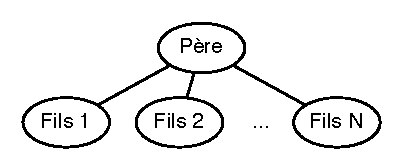
\includegraphics[scale=.5]{images/Nfils}
\end{figurehere}

\textbf{Un processus créé $N$ descendants}\\
\lstinline!for(i=0; (i<N) && ((pid = fork())==0); i++);!
\begin{figurehere}
    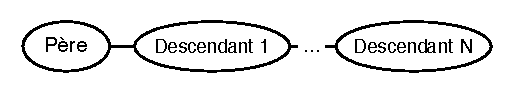
\includegraphics[scale=.5]{images/Ndesc}
\end{figurehere}

\vskip 5pt
\textbf{Modification du handler associé à \lstinline!SIGINT!}
\begin{BlockIndent}
\vspace{-5pt}\begin{lstlisting}
void sig_hand(int sig){
	printf("Signal %d.\n", sig);
}
...
struct sigaction action, old;
sigemptyset(&action.sa_mask);
action.sa_flags = 0;
action.sa_handler = sig_hand;
sigaction(SIGINT, &action, &old);
\end{lstlisting}\vspace{-5pt}
\end{BlockIndent}

\vskip 5pt
\textbf{Masquer le signal \lstinline!SIGINT!}

\begin{figurehere}
	\vspace{-5pt}
    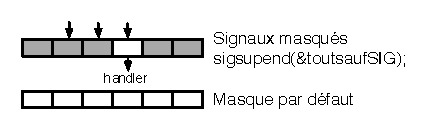
\includegraphics[scale=.75]{images/bloquer-sig}
	\vspace{-7pt}
\end{figurehere}

\begin{BlockIndent}
\vspace{-5pt}\begin{lstlisting}
sigset_t queSIGINT, old;
sigemptyset(&queSIGINT);
sigaddset(&queSIGINT, SIGINT);
sigprocmask(SIG_SETMASK, &queSIGINT, &old);
/* Actions avec SIGINT masque */
sigprocmask(SIG_SETMASK, &old, NULL);
\end{lstlisting}\vspace{-5pt}
\end{BlockIndent}

\vskip 5pt
\textbf{Se bloquer en attente du signal \lstinline!SIGINT!}

\begin{figurehere}
	\vspace{-5pt}
    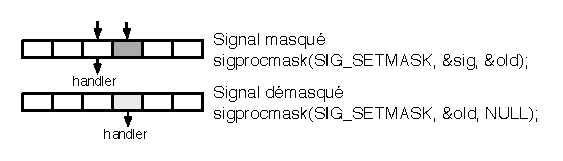
\includegraphics[scale=.75]{images/masquer-signal}
	\vspace{-7pt}
\end{figurehere}
\begin{BlockIndent}
\vspace{-5pt}\begin{lstlisting}
sigset_t toutsaufSIGINT;
sigfillset(&toutsaufSIGINT);
sigdelset(&toutsaufSIGINT, SIGINT);
//Attente du signal SIGINT
sigsupend(&toutsaufSIGINT);
\end{lstlisting}\vspace{-5pt}
\end{BlockIndent}

\vskip 5pt
\textbf{Créer un fichier vide}\\
Ouvre un fichier pour l'écriture, créé le fichier s'il n'existe pas, sinon le système vide le fichier déjà existant.
\begin{BlockIndent}
\vspace{-5pt}\begin{lstlisting}
int fd;
char *filename = "/tmp/file";
int flags = O_WRONLY | O_CREAT | O_TRUNC;
mode_t mode = S_IRUSR | S_IWUSR | S_IRGRP | S_IROTH;
if((fd = open(filename, flags, mode)) == -1) {
    perror("open"); exit(1);
}
\end{lstlisting}\vspace{-5pt}
\end{BlockIndent}

\columnbreak
\vskip 5pt
\textbf{Test de l'existence d'un fichier}\begin{itemize}
	\item Avec \lstinline!stat()! :
\vspace{-5pt}\begin{lstlisting}
struct stat stat_info;
char *filename = "/tmp/file";
if(stat(filename, &stat_info) == -1){
	if(errno == ENOENT){
		printf("%s already exists\n", filename);
	} else {
		perror("stat error");
		exit(EXIT_FAILURE);
	}
}
\end{lstlisting}\vspace{-5pt}
	\item Avec \lstinline!access()! :
\vspace{-5pt}\begin{lstlisting}
char *filename = "/tmp/file";
if(access(filename, F_OK) == -1) {
	if(errno == ENOENT) {
		printf("%s already exists\n", filename);
	} else {
		perror("access error");
		exit(EXIT_FAILURE);
	}
}
\end{lstlisting}\vspace{-5pt}
	\item Avec \lstinline!open()! (\textbf{déconseillé}) :
	\vspace{-5pt}\begin{lstlisting}
int fd;
char *filename = "/tmp/file";
int flags = O_WRONLY | O_CREAT | O_EXCL;
mode_t mode = S_IRUSR | S_IWUSR | S_IRGRP | S_IROTH;
if((fd = open(filename, flags, mode)) == -1) {
	if(errno == EEXIST) {
		printf("Ouput file exists\n");
	} else {
		perror("open");
		exit(EXIT_FAILURE);
	}
}
\end{lstlisting}\vspace{-5pt}
\end{itemize}

\vskip 5pt
\textbf{Créer un tube nommé en lecture}

\begin{figurehere}
    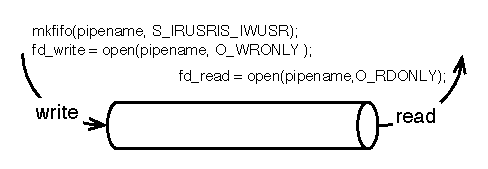
\includegraphics[scale=.75]{images/pipe-nomm}
\end{figurehere}
\begin{BlockIndent}
\vspace{-5pt}\begin{lstlisting}
int fd;
char *pipename = "pipe";

// ECRIVAIN
if(mkfifo(pipename, S_IRUSR|S_IWUSR) == -1){
	perror("mkfifo error");
	exit(EXIT_FAILURE);
}
if((fd = open(pipename, O_WRONLY)) == -1) {
	perror("open error O_WRONLY");
	exit(EXIT_FAILURE);
}

// LECTEUR
if((fd = open(pipename, O_RDONLY)) == -1) {
	perror("open error O_RDONLY");
	exit(EXIT_FAILURE);
}
\end{lstlisting}\vspace{-5pt}
\end{BlockIndent}

\vbox{
\vskip 5pt
\textbf{Création d'un tube anonyme}

\begin{figurehere}
    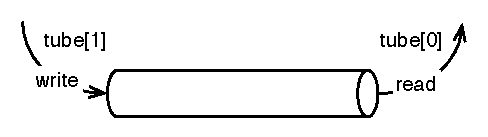
\includegraphics[scale=.75]{images/pipe-anon}
\end{figurehere}
\begin{BlockIndent}
\vspace{-5pt}\begin{lstlisting}
int tube[2];
pid_t pid_fils;
struct results res;
if(pipe(tube) == -1) {
	perror("pipe");
	exit(EXIT_FAILURE);
}
if((pid_fils = fork()) == 0){ //fils, ecriture
	/* construction de res */
	if(write(tube[1], res, sizeof(res)) == -1){
		perror("write pipe");
		exit(EXIT_FAILURE);
	}
	close(tube[1]);
} else if(pid_fils > 0) { //pere, lecture
	if(read(tube[1], res, sizeof(res)) == -1){
		perror("read pipe");
		exit(EXIT_FAILURE);
	}
	/* traitements sur res */
	close(tube[0]);
} else {
	perror("fork");
	exit(EXIT_FAILURE);
}
\end{lstlisting}\vspace{-5pt}
\end{BlockIndent}
}

\vfill

\columnbreak
\vskip 5pt
\textbf{Créer un segment de mémoire partagée nommé partagé entre un client et un serveur}
\begin{enumerate}
	\item \lstinline!shm_open()! : création d'un segment de mémoire partagée de taille 0 ;
	\item \lstinline!ftruncate()! : donner une taille au segment de mémoire partagée (en cas de réduction du segment de mémoire partagé, seul le surplus est détruit) ;
	\item \lstinline!mmap()! : mapper le segment de mémoire partagée dans l'espace d'adressage du processus.
\end{enumerate}
\begin{BlockIndent}
\vspace{-5pt}\begin{lstlisting}
struct shm_data * sp;
int fd_shm;
char * shm_name = "SHM";

// SERVEUR
//Ouverture shm
if((fd_shm = shm_open(shm_name, O_RDWR|O_CREAT, 0600)) == -1) {
	perror("shm_open error");
	exit(EXIT_FAILURE);
}

//Allocation d'une taille au shm
if(ftruncate(fd_shm, sizeof(struct shm_data)) == -1) {
	perror("ftruncate error");
	exit(EXIT_FAILURE);
}

//Mapping du shm
if((sp = mmap(NULL, sizeof(struct shm_data), PROT_READ|PROT_WRITE, MAP_SHARED, fd_shm, 0)) == MAP_FAILED) {
	perror("mmap error");
	exit(EXIT_FAILURE);
}

// CLIENT
//Ouverture du shm cree par le serveur
if((fd_shm = shm_open(shm_name, O_RDWR, 0600)) == -1) {
	perror("shm_open error");
	exit(EXIT_FAILURE);
}

//Mapping du shm ouvert
if((sp = mmap(NULL, sizeof(struct shm_data), PROT_READ|PROT_WRITE, MAP_SHARED, fd_shm, 0)) == MAP_FAILED) {
	perror("mmap error");
	exit(EXIT_FAILURE);
}
\end{lstlisting}\vspace{-5pt}
\end{BlockIndent}

\columnbreak
\vskip 5pt
\textbf{Créer un segment de mémoire partagée anonyme}
\begin{enumerate}
	\item \lstinline!mmap()! avec les arguments \lstinline!flags = MAP_ANONYMOUS! et \lstinline!fd = -1!.
\end{enumerate}

Plusieurs variables partagées $\Rightarrow$ Déclarer une structure \lstinline!struct shared_data! contenant les variables partagées.\\
\textbf{Attention.} Cas des structures de structures avec les pointeurs de structures (la structure pointée ne se trouve pas dans la mémoire partagée, contrairement au pointeur).

\begin{figurehere}
    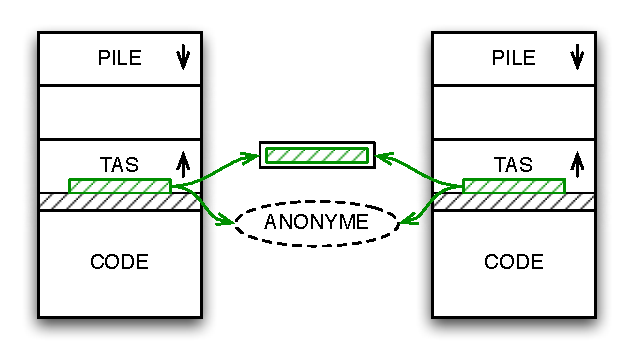
\includegraphics[scale=.6]{images/mmap}
\end{figurehere}

\vskip 5pt
\textbf{Redéfinition du handler de \lstinline!SIGINT! pour fermer les structures ouvertes avant de les ouvrir}\\
Dans le code du handler : \lstinline&if(fd != NULL) close(fd);&

\vskip 5pt
\textbf{Sémaphore anonyme}\\
Utilisation avec un segment de mémoire partagée anonyme. Le sémaphore est alors partagé entre le père et sa descendance.
\begin{BlockIndent}
\vspace{-5pt}\begin{lstlisting}
sem_t * sem;
if((sem = mmap(NULL, sizeof(sem_t), PROT_READ|PROT_WRITE, MAP_ANONYMOUS|MAP_SHARED, -1, 0)) == MAP_FAILED) {
	perror("mmap anonymous error");
	exit(EXIT_FAILURE);
}
//Ouverture du semaphore de synchronisation entre le pere et les fils
if(sem_init(sem, 1, 0) == -1) {
	perror("sem_init error");
	exit(EXIT_FAILURE);
}
\end{lstlisting}\vspace{-5pt}
\end{BlockIndent}

\vskip 5pt
\textbf{Emplacement des sémaphores et segments de mémoire partagée}\\
Placés dans le répertoire \lstinline!/dev/shm! dans les distributions Linux.

\vskip 5pt
\textbf{Différents états d'un processus}

\begin{figurehere}
    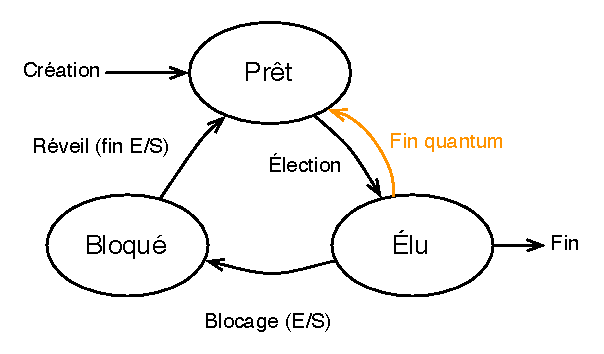
\includegraphics[scale=.6]{images/etat-process-split-time}
\end{figurehere}

\columnbreak
\textbf{Segments d'un processus}

\begin{figurehere}
    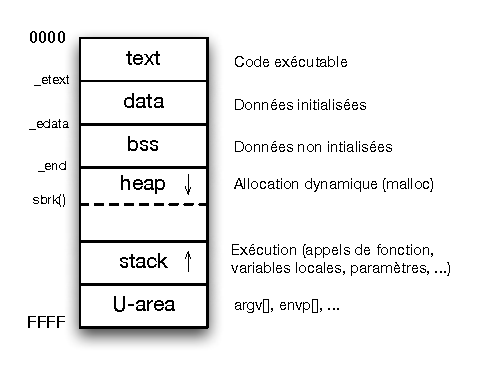
\includegraphics[scale=.7]{images/process-seg}
\end{figurehere}

\textbf{Etats d'un processus}

\begin{figurehere}
    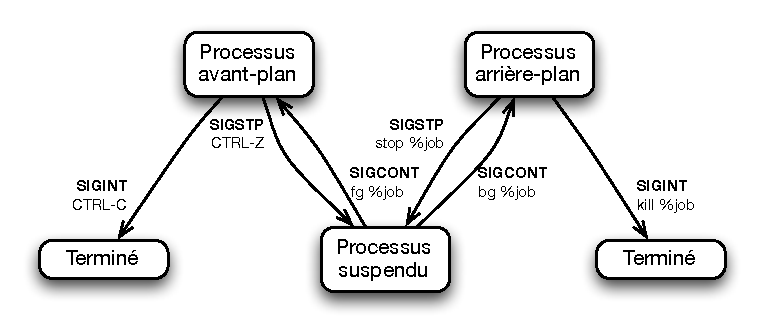
\includegraphics[scale=.6]{images/process-state}
\end{figurehere}

\textbf{Descripteurs de fichier}\\

\begin{figurehere}
    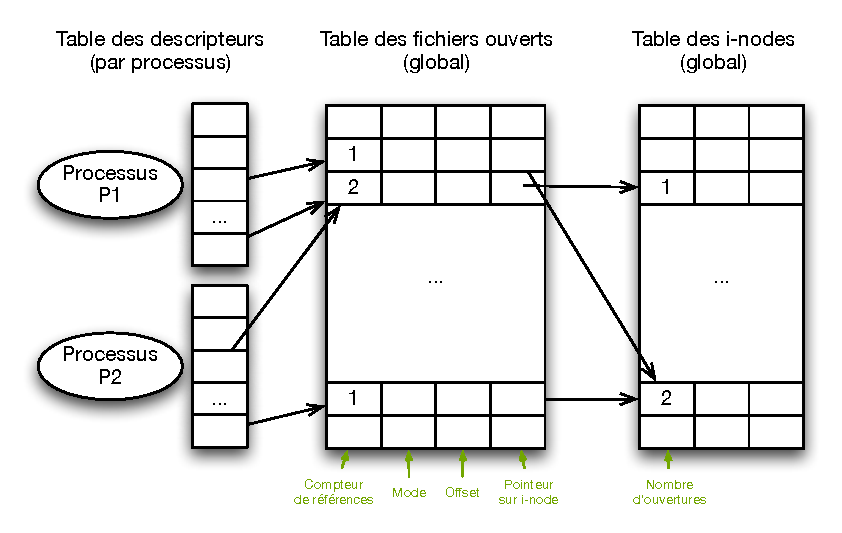
\includegraphics[scale=.6]{images/descripteurs.pdf}
\end{figurehere}

\vskip 5pt
\textbf{Synchronisation sans sémaphores}\\
Utilisation d'un anneau où un signal part de la source et se propage jusqu'à atteindre la source. Il est impossible de compter le nombre de signaux qui arrivent à la source.\\
Problème de performance : plus de parallélisme.
\begin{figurehere}
    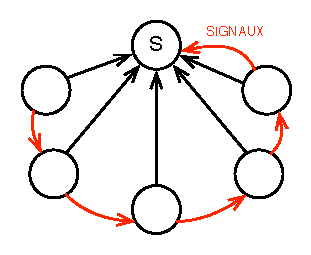
\includegraphics[scale=.7]{images/anneau}
\end{figurehere}

\end{multicols}



\clearpage
\head{ERRNO ERRORS}
\vspace{-5pt}\begin{lstlisting}[multicols=2]
Fichier /usr/include/asm-generic/errno-base.h

#ifndef _ASM_GENERIC_ERRNO_BASE_H 
#define _ASM_GENERIC_ERRNO_BASE_H  

#define EPERM 1 /* Operation not permitted */ 
#define ENOENT 2 /* No such file or directory */
#define ESRCH 3 /* No such process */ 
#define EINTR 4 /* Interrupted system call */ 
#define EIO 5 /* I/O error */ 
#define ENXIO 6 /* No such device or address */
#define E2BIG 7 /* Argument list too long */ 
#define ENOEXEC 8 /* Exec format error */ 
#define EBADF 9 /* Bad file number */ 
#define ECHILD 10 /* No child processes */ 
#define EAGAIN 11 /* Try again */ 
#define ENOMEM 12 /* Out of memory */ 
#define EACCES 13 /* Permission denied */ 
#define EFAULT 14 /* Bad address */ 
#define ENOTBLK 15 /* Block device required */ 
#define EBUSY 16 /* Device or resource busy */ 
#define EEXIST 17 /* File exists */ 
#define EXDEV 18 /* Cross-device link */ 
#define ENODEV 19 /* No such device */ 
#define ENOTDIR 20 /* Not a directory */ 
#define EISDIR 21 /* Is a directory */
#define EINVAL 22 /* Invalid argument */ 
#define ENFILE 23 /* File table overflow */ 
#define EMFILE 24 /* Too many open files */ 
#define ENOTTY 25 /* Not a typewriter */ 
#define ETXTBSY 26 /* Text file busy */ 
#define EFBIG 27 /* File too large */ 
#define ENOSPC 28 /* No space left on device */ 
#define ESPIPE 29 /* Illegal seek */ 
#define EROFS 30 /* Read-only file system */ 
#define EMLINK 31 /* Too many links */ 
#define EPIPE 32 /* Broken pipe */ 
#define EDOM 33 /* Math argument out of domain of func */ 
#define ERANGE 34 /* Math result not representable */ 

#endif 


Fichier /usr/include/asm-generic/errno.h

#ifndef _ASM_GENERIC_ERRNO_H 
#define _ASM_GENERIC_ERRNO_H  

#include <asm-generic/errno-base.h>  

#define EDEADLK 35 /* Resource deadlock would occur */ 
#define ENAMETOOLONG 36 /* File name too long */ 
#define ENOLCK 37 /* No record locks available */ 
#define ENOSYS 38 /* Function not implemented */ 
#define ENOTEMPTY 39 /* Directory not empty */ 
#define ELOOP 40 /* Too many symbolic links encountered */ 
#define EWOULDBLOCK EAGAIN /* Operation would block */ 
#define ENOMSG 42 /* No message of desired type */ 
#define EIDRM 43 /* Identifier removed */ 
#define ECHRNG 44 /* Channel number out of range */ 
#define EL2NSYNC 45 /* Level 2 not synchronized */ 
#define EL3HLT 46 /* Level 3 halted */ 
#define EL3RST 47 /* Level 3 reset */ 
#define ELNRNG 48 /* Link number out of range */ 
#define EUNATCH 49 /* Protocol driver not attached */ 
#define ENOCSI 50 /* No CSI structure available */ 
#define EL2HLT 51 /* Level 2 halted */ 
#define EBADE 52 /* Invalid exchange */ 
#define EBADR 53 /* Invalid request descriptor */ 
#define EXFULL 54 /* Exchange full */ 
#define ENOANO 55 /* No anode */ 
#define EBADRQC 56 /* Invalid request code */ 
#define EBADSLT 57 /* Invalid slot */  

#define EDEADLOCK EDEADLK  

#define EBFONT 59 /* Bad font file format */ 
#define ENOSTR 60 /* Device not a stream */ 
#define ENODATA 61 /* No data available */ 
#define ETIME 62 /* Timer expired */ 
#define ENOSR 63 /* Out of streams resources */ 
#define ENONET 64 /* Machine is not on the network */ 
#define ENOPKG 65 /* Package not installed */ 
#define EREMOTE 66 /* Object is remote */ 
#define ENOLINK 67 /* Link has been severed */ 
#define EADV 68 /* Advertise error */ 
#define ESRMNT 69 /* Srmount error */ 
#define ECOMM 70 /* Communication error on send */ 
#define EPROTO 71 /* Protocol error */ 
#define EMULTIHOP 72 /* Multihop attempted */ 
#define EDOTDOT 73 /* RFS specific error */ 
#define EBADMSG 74 /* Not a data message */ 
#define EOVERFLOW 75 /* Value too large for defined data type */ 
#define ENOTUNIQ 76 /* Name not unique on network */ 
#define EBADFD 77 /* File descriptor in bad state */ 
#define EREMCHG 78 /* Remote address changed */ 
#define ELIBACC 79 /* Can not access a needed shared library */ 
#define ELIBBAD 80 /* Accessing a corrupted shared library */ 
#define ELIBSCN 81 /* .lib section in a.out corrupted */ 
#define ELIBMAX 82 /* Attempting to link in too many shared libraries */ 
#define ELIBEXEC 83 /* Cannot exec a shared library directly */ 
#define EILSEQ 84 /* Illegal byte sequence */ 
#define ERESTART 85 /* Interrupted system call should be restarted */ 
#define ESTRPIPE 86 /* Streams pipe error */ 
#define EUSERS 87 /* Too many users */ 
#define ENOTSOCK 88 /* Socket operation on non-socket */ 
#define EDESTADDRREQ 89 /* Destination address required */ 
#define EMSGSIZE 90 /* Message too long */ 
#define EPROTOTYPE 91 /* Protocol wrong type for socket */ 
#define ENOPROTOOPT 92 /* Protocol not available */ 
#define EPROTONOSUPPORT 93 /* Protocol not supported */ 
#define ESOCKTNOSUPPORT 94 /* Socket type not supported */ 
#define EOPNOTSUPP 95 /* Operation not supported on transport endpoint */ 
#define EPFNOSUPPORT 96 /* Protocol family not supported */ 
#define EAFNOSUPPORT 97 /* Address family not supported by protocol */ 
#define EADDRINUSE 98 /* Address already in use */ 
#define EADDRNOTAVAIL 99 /* Cannot assign requested address */ 
#define ENETDOWN 100 /* Network is down */ 
#define ENETUNREACH 101 /* Network is unreachable */ 
#define ENETRESET 102 /* Network dropped connection because of reset */ 
#define ECONNABORTED 103 /* Software caused connection abort */ 
#define ECONNRESET 104 /* Connection reset by peer */ 
#define ENOBUFS 105 /* No buffer space available */ 
#define EISCONN 106 /* Transport endpoint is already connected */ 
#define ENOTCONN 107 /* Transport endpoint is not connected */ 
#define ESHUTDOWN 108 /* Cannot send after transport endpoint shutdown */ 
#define ETOOMANYREFS 109 /* Too many references: cannot splice */ 
#define ETIMEDOUT 110 /* Connection timed out */ 
#define ECONNREFUSED 111 /* Connection refused */ 
#define EHOSTDOWN 112 /* Host is down */ 
#define EHOSTUNREACH 113 /* No route to host */ 
#define EALREADY 114 /* Operation already in progress */ 
#define EINPROGRESS 115 /* Operation now in progress */ 
#define ESTALE 116 /* Stale NFS file handle */ 
#define EUCLEAN 117 /* Structure needs cleaning */ 
#define ENOTNAM 118 /* Not a XENIX named type file */ 
#define ENAVAIL 119 /* No XENIX semaphores available */ 
#define EISNAM 120 /* Is a named type file */ 
#define EREMOTEIO 121 /* Remote I/O error */ 
#define EDQUOT 122 /* Quota exceeded */  

#define ENOMEDIUM 123 /* No medium found */ 
#define EMEDIUMTYPE 124 /* Wrong medium type */ 
#define ECANCELED 125 /* Operation Canceled */ 
#define ENOKEY 126 /* Required key not available */ 
#define EKEYEXPIRED 127 /* Key has expired */ 
#define EKEYREVOKED 128 /* Key has been revoked */ 
#define EKEYREJECTED 129 /* Key was rejected by service */  

/* for robust mutexes */
#define EOWNERDEAD 130 /* Owner died */ 
#define ENOTRECOVERABLE 131 /* State not recoverable */  

#endif
\end{lstlisting}\vspace{-5pt}

\end{document}
